
\RequirePackage{currfile} 
\documentclass{beamer}



%%%%%%%%%%%%%% PACKAGES %%%%%%%%%%%%%%%%%%%%%
\usepackage{textpos}   
\usepackage{graphicx} % Allows including images
\usepackage{booktabs} % Allows the use of \toprule, \midrule and \bottomrule in tables
\usepackage{biblatex} % Allows for \cite 
\usepackage[utf8]{inputenc}
\usepackage{tikz} \usetikzlibrary{calc, arrows.meta, intersections, patterns, positioning, shapes.misc, fadings, through,decorations.pathreplacing}
\usepackage{array} % To pause columns
\usepackage[usenames,dvipsnames]{xcolor}
\usepackage{colortbl}
\usepackage{multicol}
\usepackage{multirow}
\usepackage{caption}
\usepackage{block} %blocks for statements
\usepackage{comment}
\usepackage[absolute,overlay]{textpos}
\usepackage{forest}
\forestset{qtree/.style={for tree={parent anchor=south, 
           child anchor=north,align=center,inner sep=0pt}}}


\definecolor{ColorOne}{named}{MidnightBlue}
\definecolor{ColorTwo}{named}{Dandelion}
\definecolor{ColorThree}{named}{Plum}

\tikzstyle{descript} = [text = black,align=center, minimum height=1.8cm, align=center, outer sep=0pt,font = \footnotesize]
\tikzstyle{activity} =[align=center,outer sep=1pt]

%% Change the bg color to adjust your transition slide background color!
\newenvironment{transitionframe}{
  \setbeamercolor{background canvas}{bg=White}
  \begin{frame}}{
    \end{frame}
}

%%%%%%%%%%%%%% COMMANDS %%%%%%%%%%%%%%%%%%%%%
\newcommand{\progressbar}{%
\pgfmathsetmacro{\theta}{360/\inserttotalframenumber*\insertframenumber}
\begin{tikzpicture}[scale=0.025]
\fill[blue] (0,0) circle (9);
\fill[green] (0,0) -- (9,0) arc (0:-\theta:9);
\fill[white] (0,0) circle (5);
\node at (0,0) {\insertframenumber};
\end{tikzpicture}
}

%%% TIKZ STUFF
\tikzset{   
        every picture/.style={remember picture,baseline},
        every node/.style={anchor=base,align=center,outer sep=1.5pt},
        every path/.style={thick},
        }
\newcommand\marktopleft[1]{%
    \tikz[overlay,remember picture] 
        \node (marker-#1-a) at (-.3em,.3em) {};%
}
\newcommand\markbottomright[2]{%
    \tikz[overlay,remember picture] 
        \node (marker-#1-b) at (0em,0em) {};%
}
\tikzstyle{every picture}+=[remember picture] 
\tikzstyle{mybox} =[draw=black, very thick, rectangle, inner sep=10pt, inner ysep=20pt]
\tikzstyle{fancytitle} =[draw=black,fill=red, text=white]
%%%% END TIKZ STUFF

%%% COLOR COLUMN (did not make it work...)
\newcolumntype{G}{>{\centering\columncolor{gray!20!white}}p{0.2\textwidth}}
\newcolumntype{C}{>{\centering\arraybackslash}p{0.2\textwidth}}
%%% END COLOR COLUMN


\AtBeginSection[]{
  \begin{frame}
  \vfill
  \centering
  \begin{beamercolorbox}[sep=8pt,center,shadow=true,rounded=true]{title}
    \usebeamerfont{title}\insertsectionhead\par%
  \end{beamercolorbox}
  \vfill
  \end{frame}
}

%%%%%%%%%%%%%%% SETTINGS %%%%%%%%%%%%%%%%%%%%%%%
\mode<presentation> {
%\usetheme{Warsaw}
%\usetheme{Frankfurt}
%\usetheme{Madrid}
\usetheme{default}
%\usecolortheme{whale}
\usecolortheme{default}
\usefonttheme{professionalfonts}
}

%To call references
%\bibliographystyle{../aea.bst}
%\bibliography{references}

%%%%%%%%%%%%%%%%%%%%%%%%%%%%%%%%%%
%FOR LINKS
\definecolor{darkblue}{rgb}{0.0, 0.0, 0.65}
\definecolor{darkgreen}{rgb}{0.0, 0.65, 0.0}
\hypersetup{
	citecolor=blue,
	colorlinks=true,
	linkcolor=blue,
	filecolor=magenta,
	urlcolor=magenta
}
%%%%%%%%%%%%%%%%%%%%%%%%%%%%%%%%%%


\setbeamertemplate{navigation symbols}{} 


%Title
\title[]{New Idea: School closures, remote learning and differential effects between only childs and children with siblings}
%\subtitle[]{DLP Writing Seminar}

\author[Francisco Pardo] % (optional, for multiple authors)
{Francisco Pardo - fpardo@utexas.edu \inst{1}}
 
\institute[UT] % (optional)
{
  \inst{1}%
  University of Texas at Austin
  %\and
  %\inst{2}%
   % ...
}

\date{\today}
 

 
 
%------------------------------------------------------------
%The next block of commands puts the table of contents at the 
%beginning of each section and highlights the current section:
%Commented because presentations are short, we don't need that. 
\begin{comment}
\AtBeginSection[]
{
  \begin{frame}
    \frametitle{Table of Contents}
    \tableofcontents[currentsection]
  \end{frame}
}
\end{comment}
%------------------------------------------------------------

\begin{document}


\frame{\titlepage}


\begin{frame}
    \label{update_scott}
    \frametitle{Some updates}
    \begin{itemize}
        \item Raw plots
        \item Single parents, sex, public schools...
        %\item No consistency when dividing by cohorts...
        \item Evidence from Netherlands
        \item Grade thresholds and Distribution. Grade imputation
        \item Dropout, employment potential?
    \end{itemize}
\end{frame}



\begin{frame}
    \label{update_scott}
    \frametitle{Some updates}
    \begin{itemize}
        \item Adjusting for grading criteria change
        \item Evidence from other countries
        \item Parallel trends
    \end{itemize}
\end{frame}


\section{Grade change criteria}

\begin{frame}
    \label{update_scott}
    \frametitle{Grade distributions pre-covid: Elementary}
 {\resizebox{0.9\textwidth}{!}{
       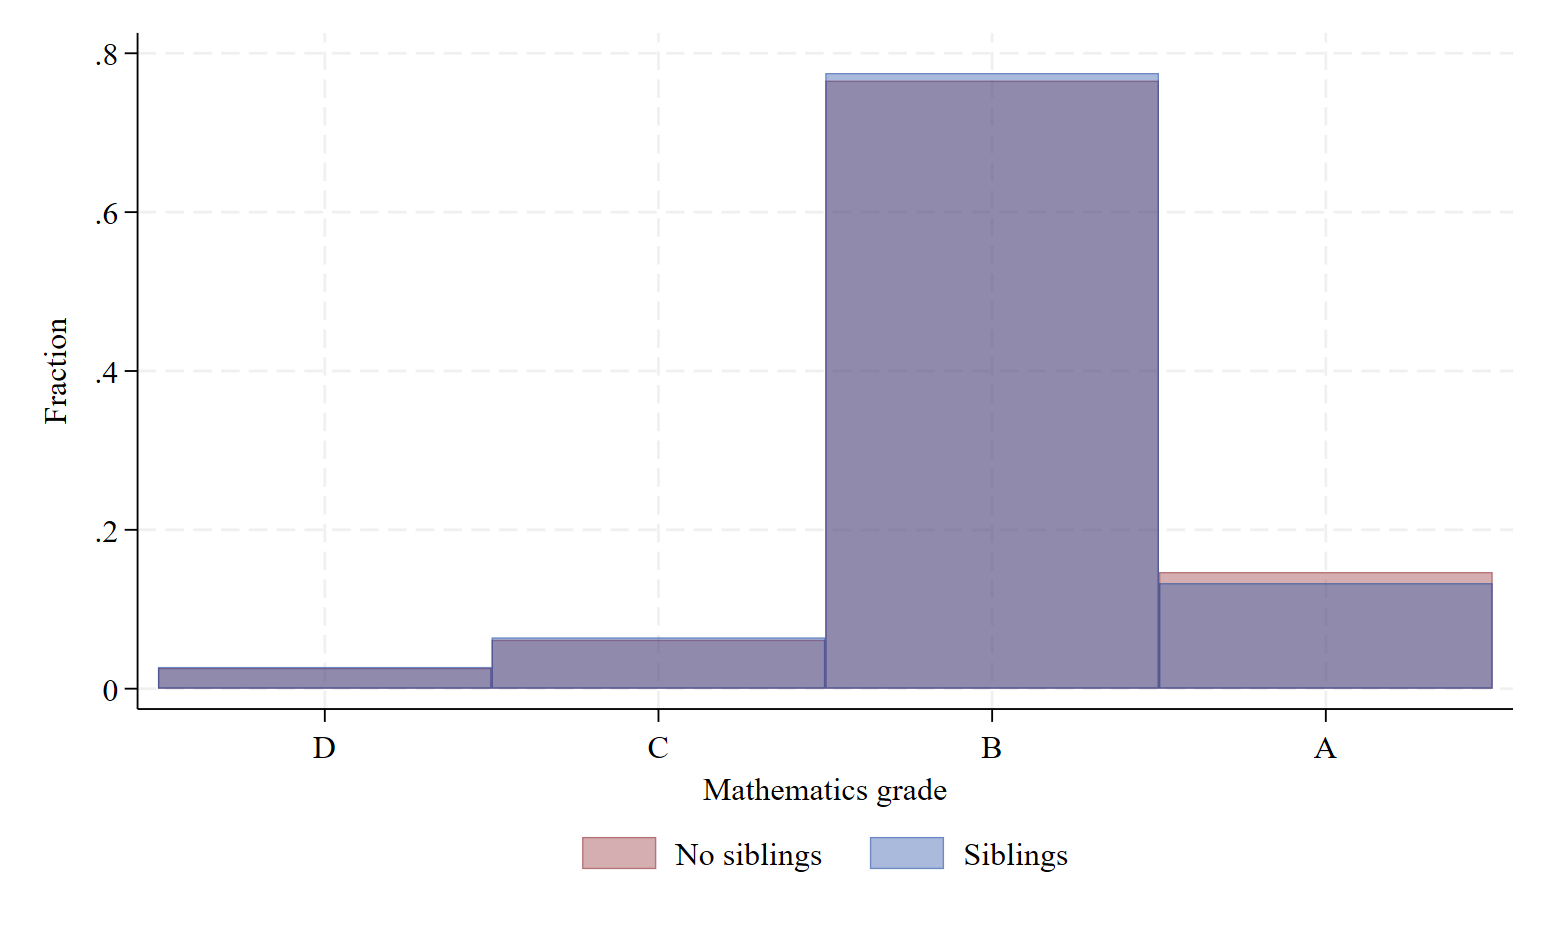
\includegraphics{./FIGURES/Descriptive/histogram_pre_elm.png}
      }
    }
\end{frame}

\begin{frame}
    \label{update_scott}
    \frametitle{Grade distributions pre-covid: Secondary}
 {\resizebox{0.9\textwidth}{!}{
       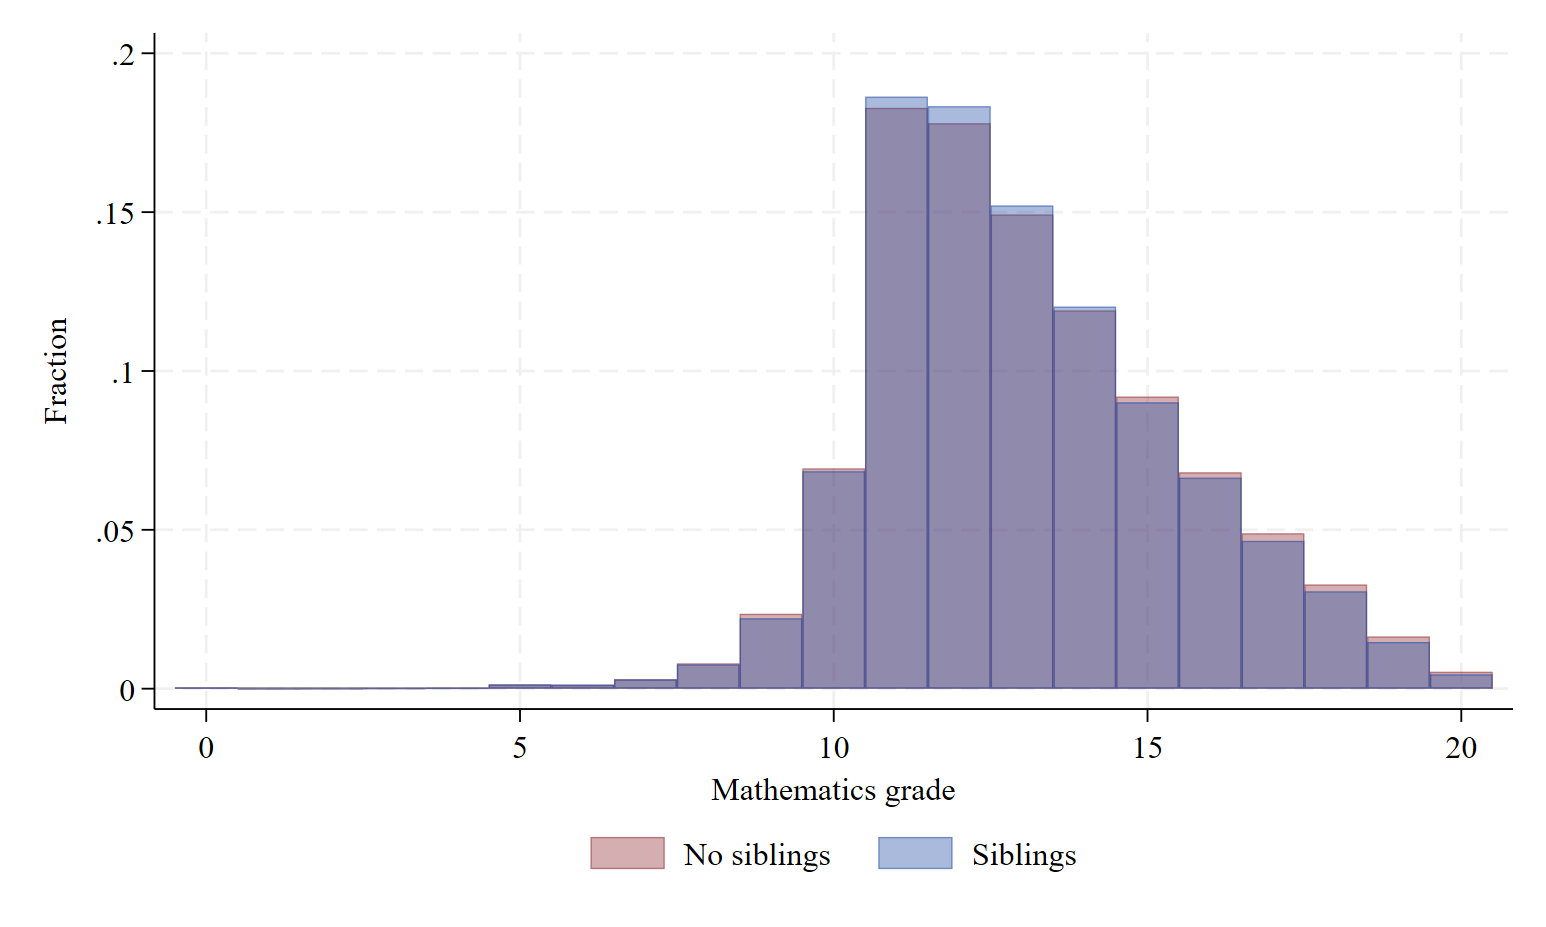
\includegraphics{./FIGURES/Descriptive/histogram_pre_9-10.png}
      }
    }
\end{frame}


\begin{frame}
    \label{update_scott}
    \frametitle{Event Study - Mathematics GPA}
        {\resizebox{0.9\textwidth}{!}{
       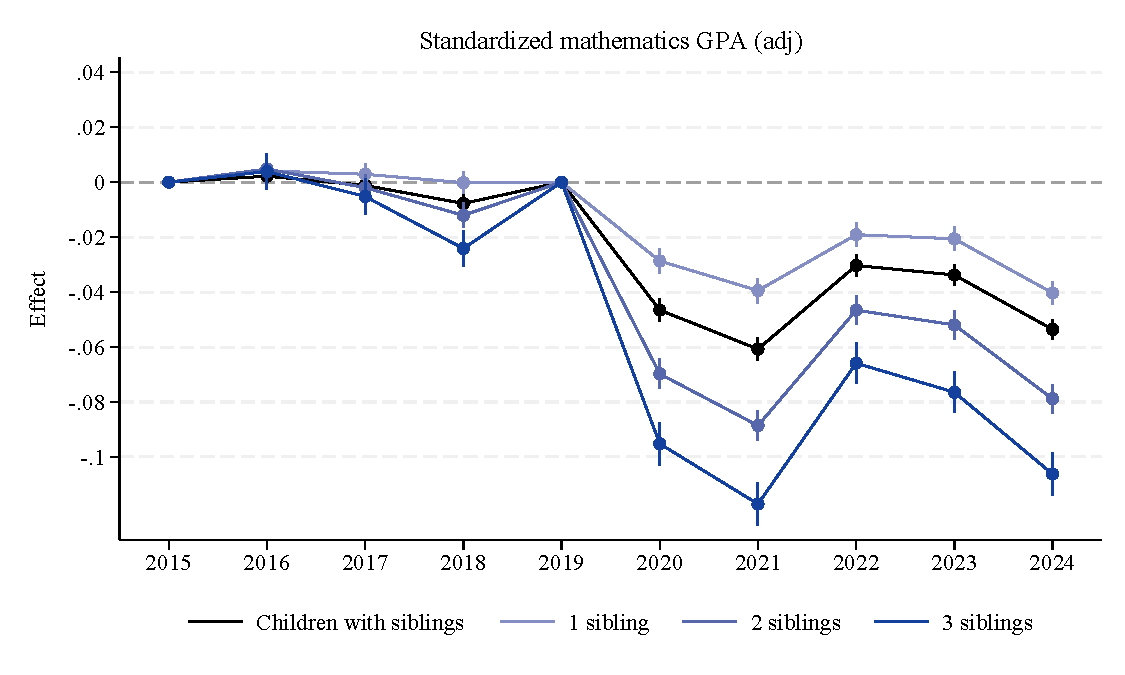
\includegraphics{./FIGURES/Event Study/covid_std_gpa_m_adj_all_all_all_elm_all.pdf}
      }
    }
\end{frame}



\section{Evidence from other countries}


\begin{frame}
    \label{update_scott}
    \frametitle{Is this just an issue in Peru?}
    \begin{itemize}
        \item Some evidence from the Netherlands suggests it is not an issue there: No heterogeneity by number of children.
        \item I need data on:
            \begin{itemize}
                \item Educational outcomes
                \item Siblings (e.g. Do you have any?, Household size, etc)
                \item pre and post covid
            \end{itemize}
    \end{itemize}
\end{frame}



\begin{frame}
    \label{update_scott}
    \frametitle{International Achievement surveys}
    \begin{itemize}
        \item PISA
            \begin{itemize}
                \item 15 y.o.
                \item 2009-2012 and 2022 allow for sibling identification
                \item 2018 includes it for some developing countries
                \item I look at countries with observations both pre-post covid
            \end{itemize}            
    \end{itemize}
\end{frame}


\begin{frame}
    \label{update_scott}
    \frametitle{PISA: From 2009/2012 to 2022}
        {\resizebox{0.9\textwidth}{!}{
       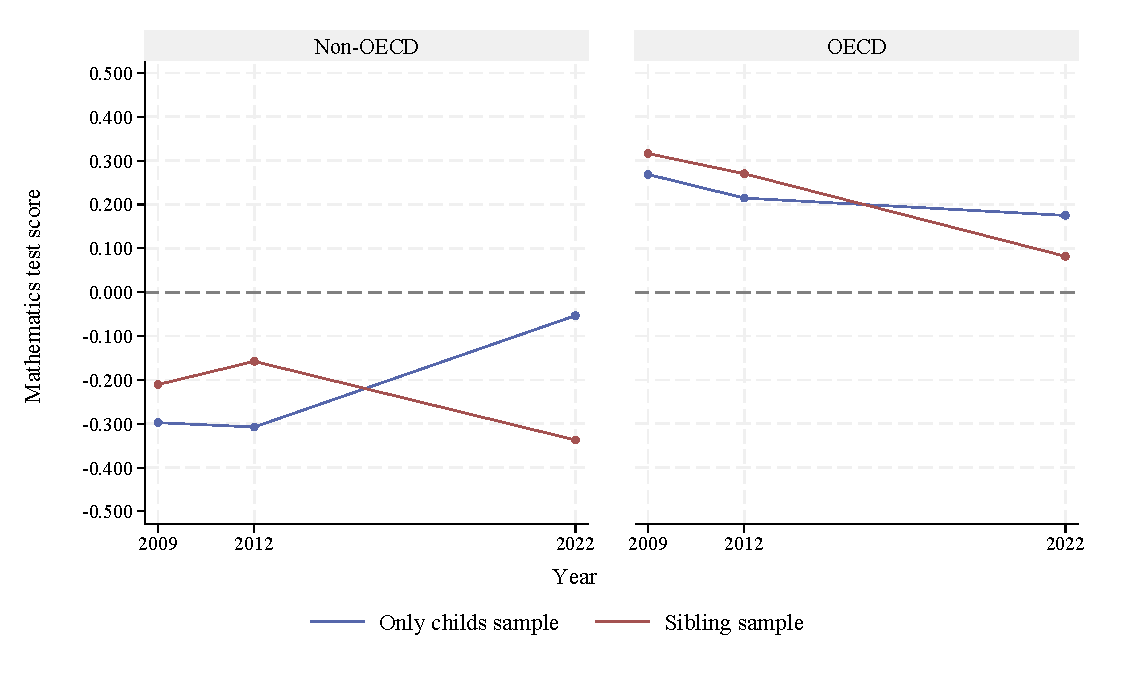
\includegraphics{./FIGURES/Descriptive/PISA_PV1MATH_2009_2022.pdf}
      }
    }
\end{frame}

\begin{frame}
    \label{update_scott}
    \frametitle{PISA-D: 2018 vs 2022}
        {\resizebox{0.9\textwidth}{!}{
       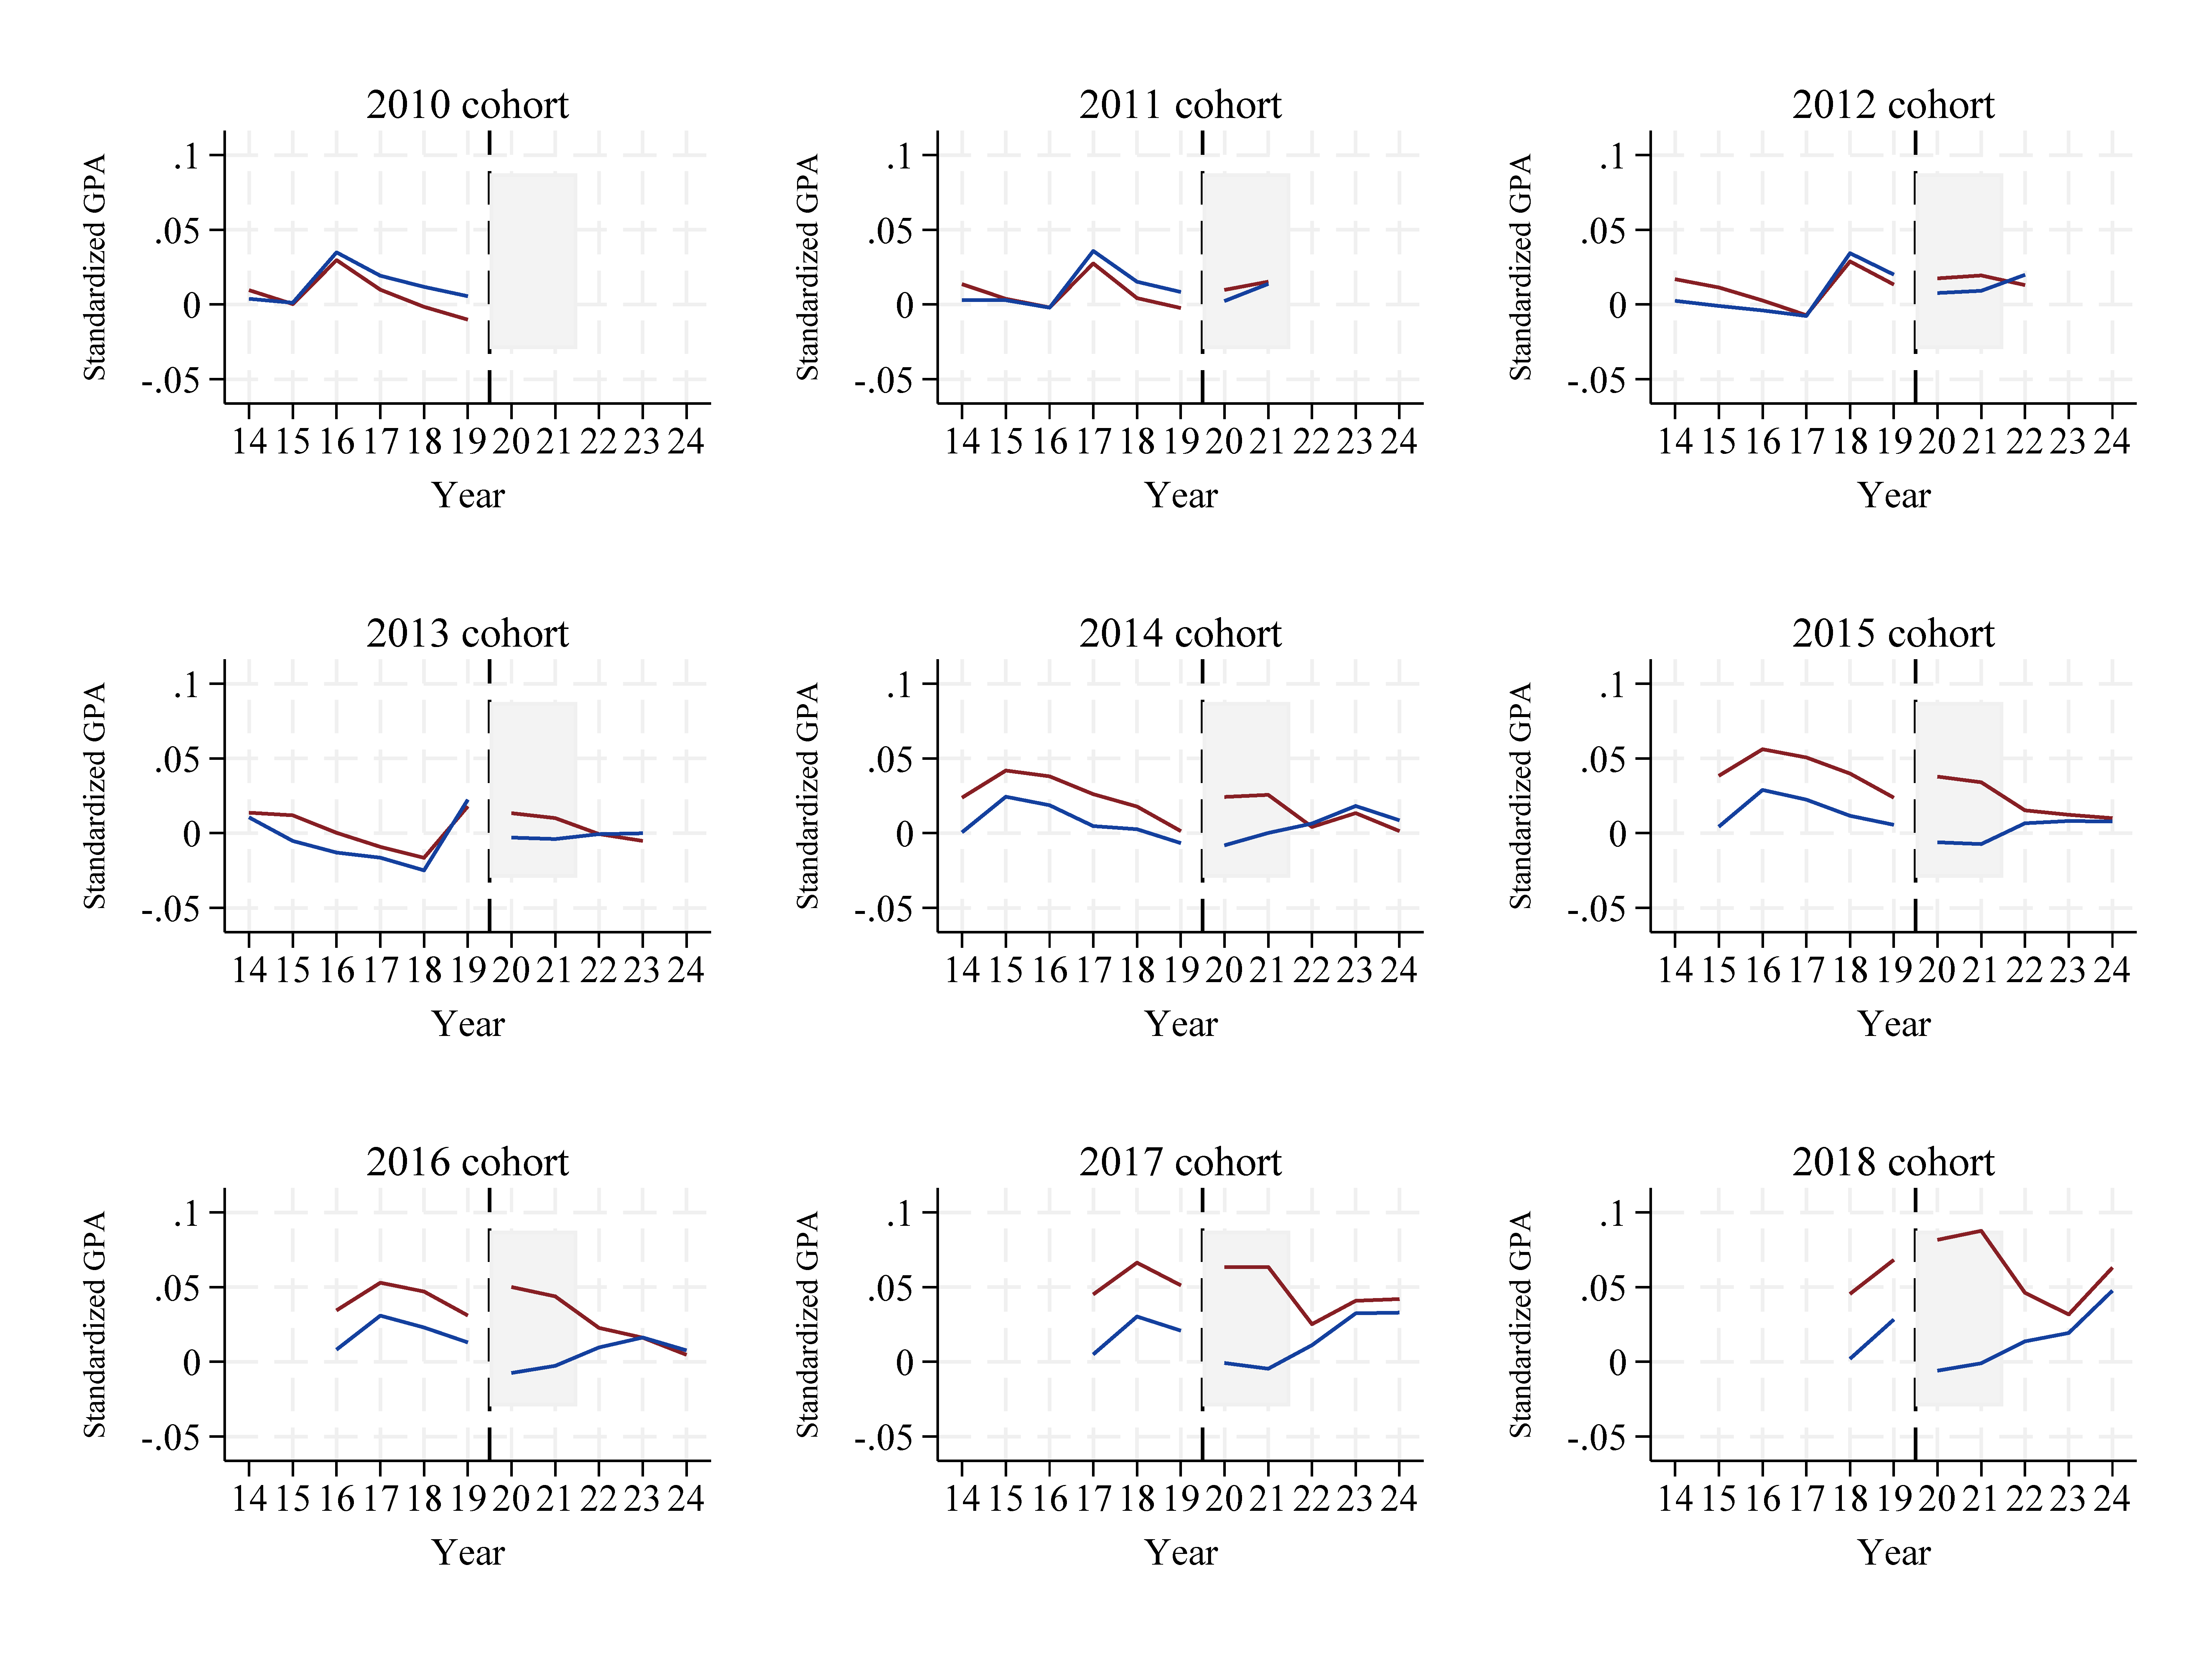
\includegraphics{./FIGURES/Descriptive/raw_cohorts_std_gpa_m.pdf}
      }
    }
\end{frame}

\begin{frame}
    \label{update_scott}
    \frametitle{MICS + FL}
        {\resizebox{0.9\textwidth}{!}{
       %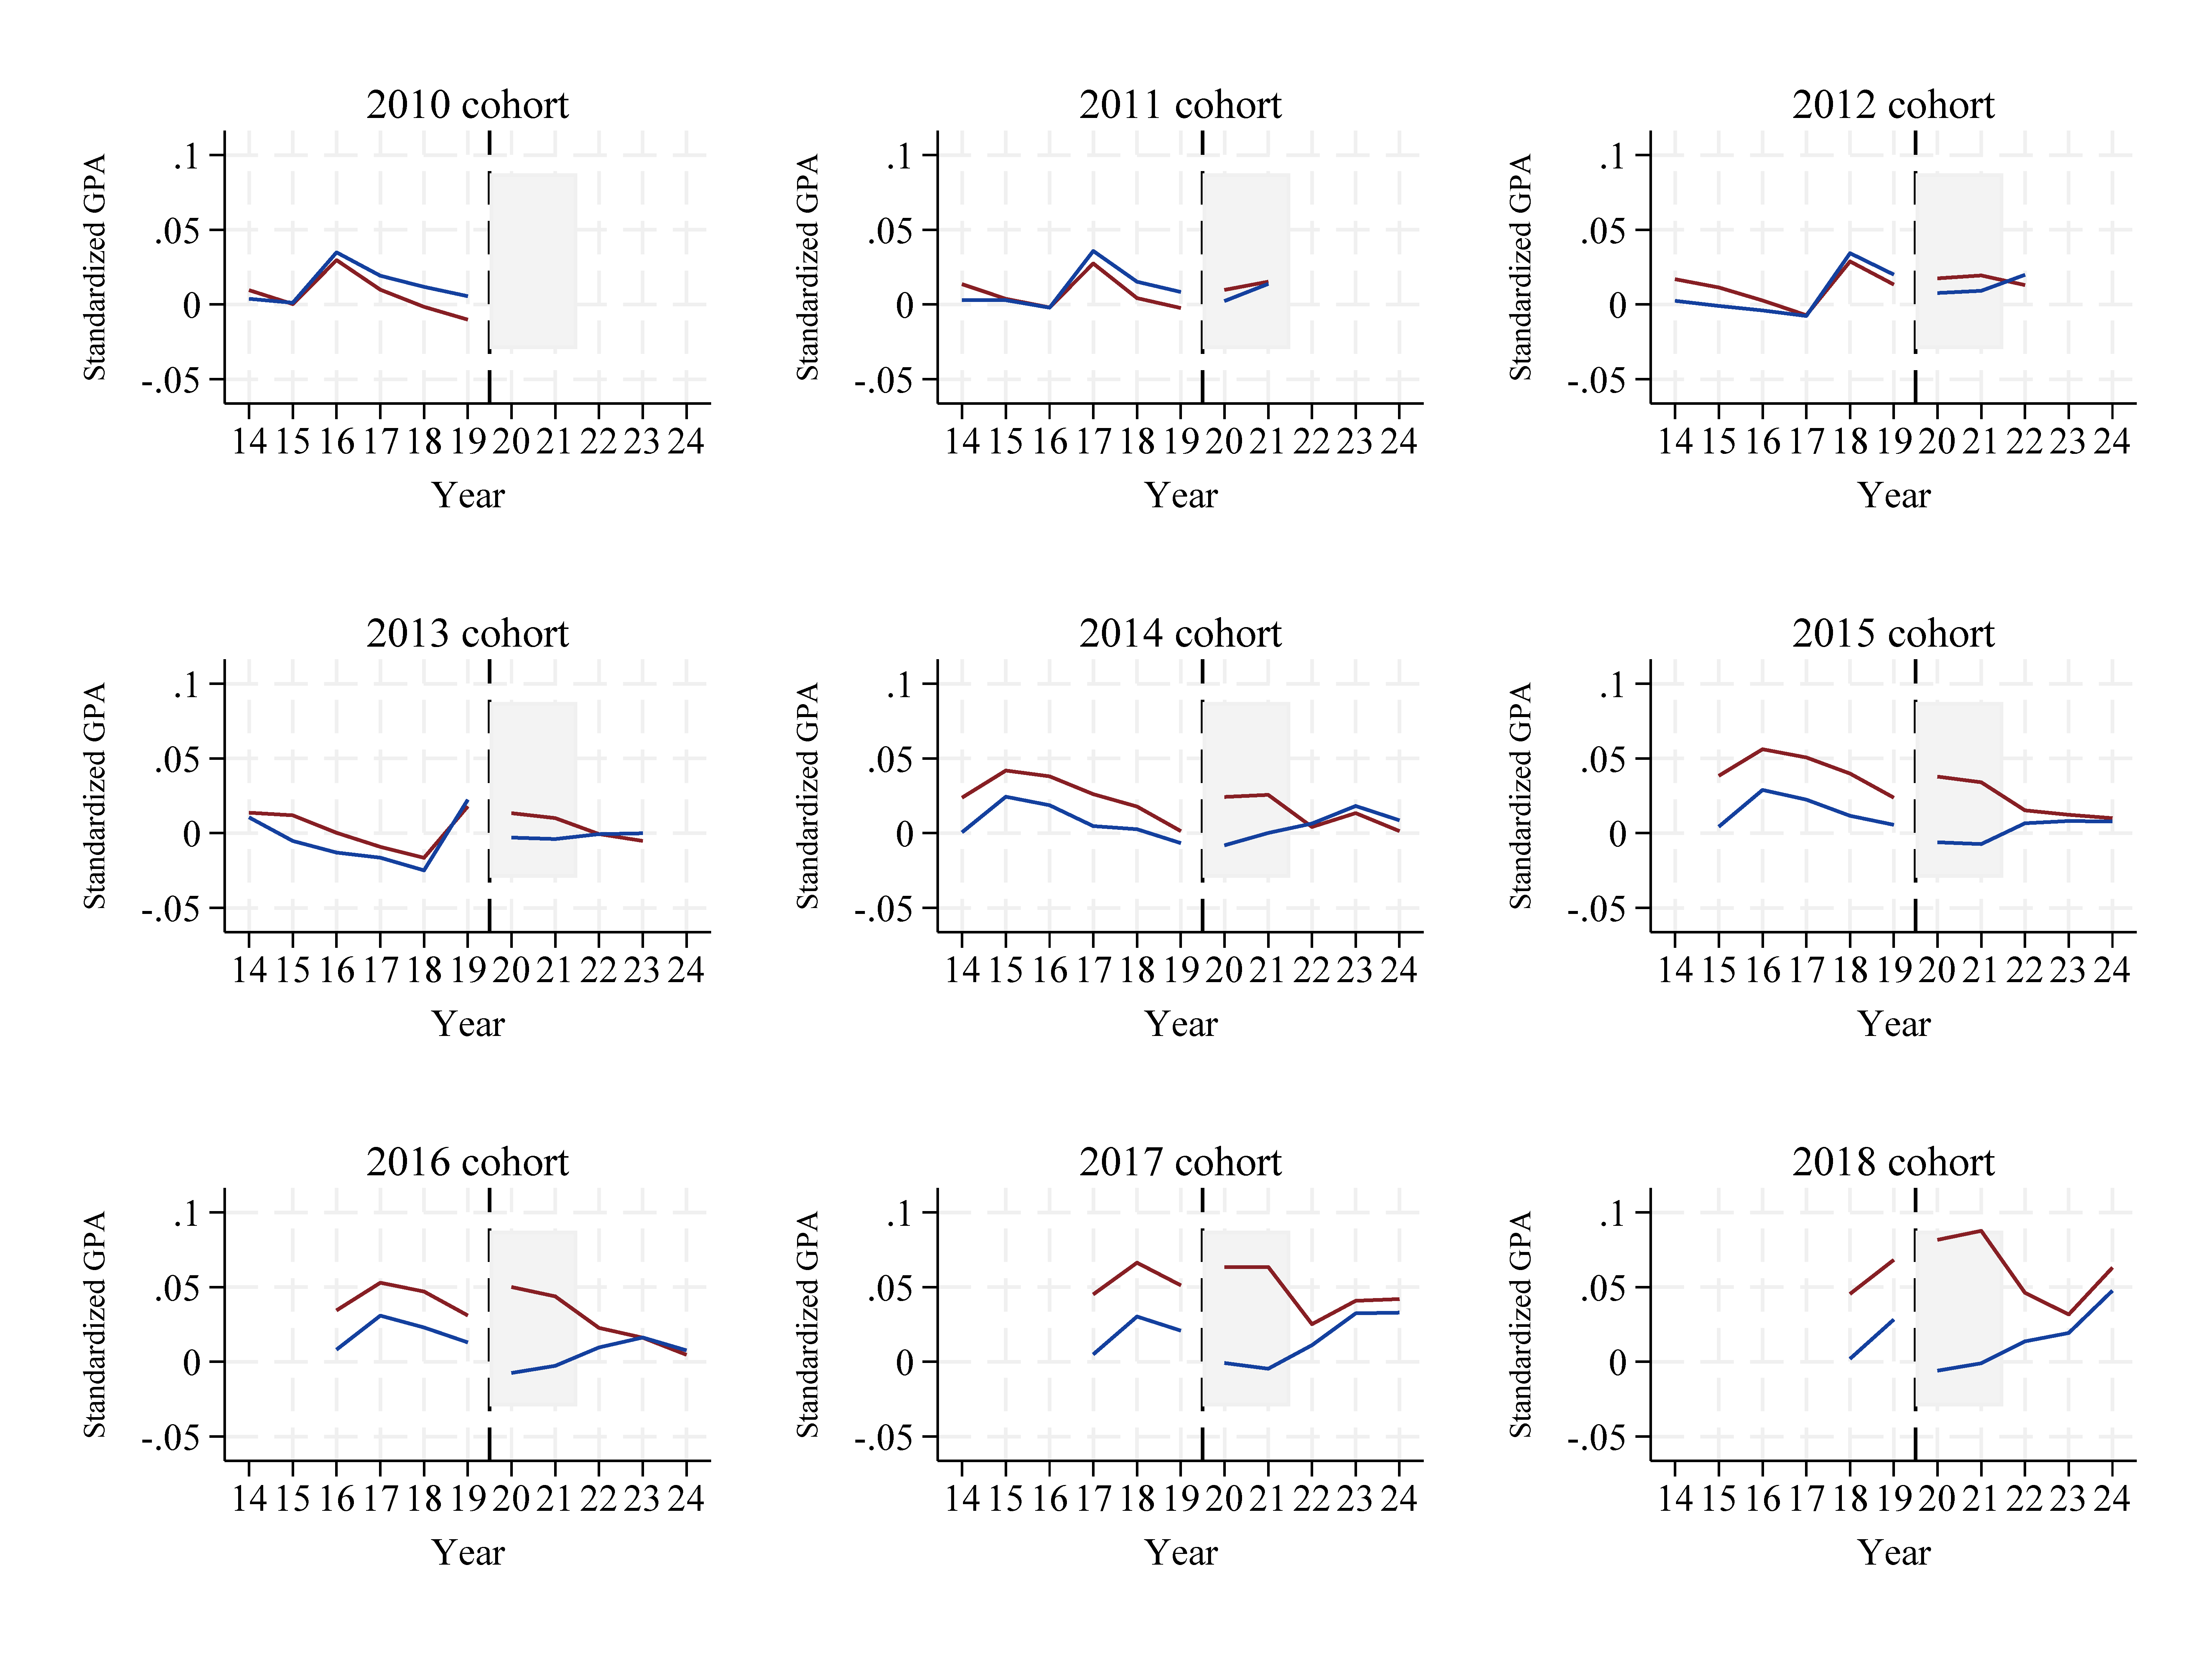
\includegraphics{./FIGURES/Descriptive/raw_cohorts_std_gpa_m.pdf}
      }
    }
\end{frame}




\section{Parallel Trends}

\begin{frame}
    \label{update_scott}
    \frametitle{\% of A's in Mathematics}
        {\resizebox{0.9\textwidth}{!}{
       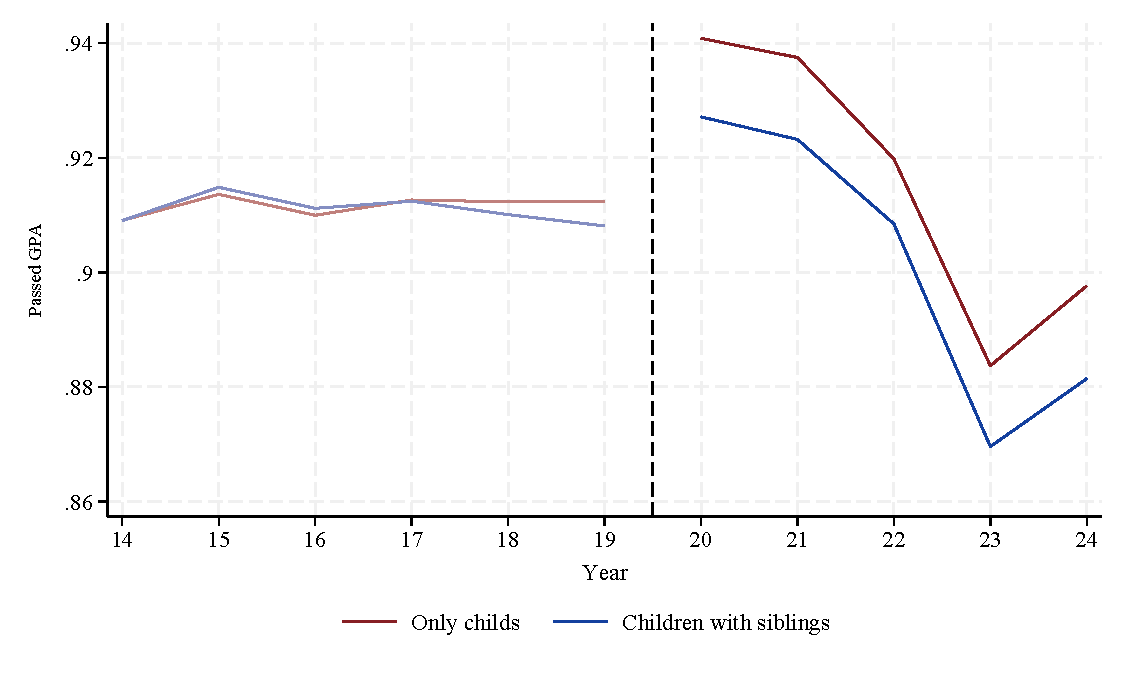
\includegraphics{./FIGURES/Descriptive/raw_total_elm_pass_math.pdf}
      }
    }
\end{frame}

\begin{frame}
    \label{update_scott}
    \frametitle{Standardized GPA in Mathematics}
        {\resizebox{0.9\textwidth}{!}{
       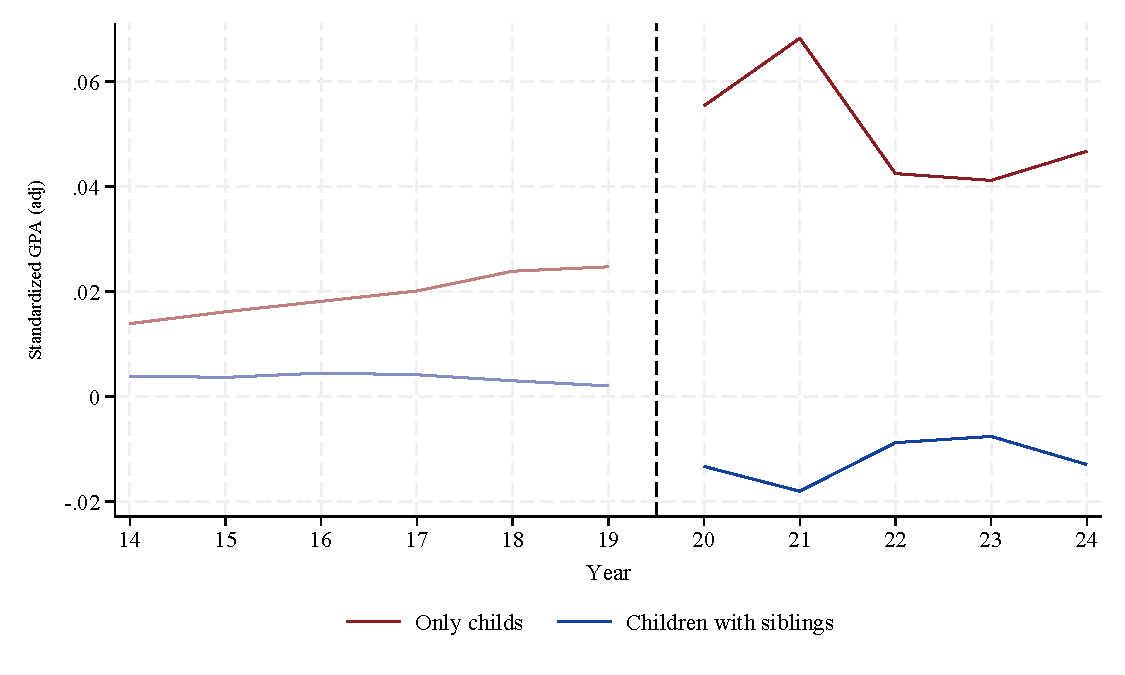
\includegraphics{./FIGURES/Descriptive/raw_total_elm_std_gpa_m_adj.pdf}
      }
    }
\end{frame}

\begin{frame}
    \label{update_scott}
    \frametitle{Standardized GPA in Mathematics}
        {\resizebox{0.9\textwidth}{!}{
       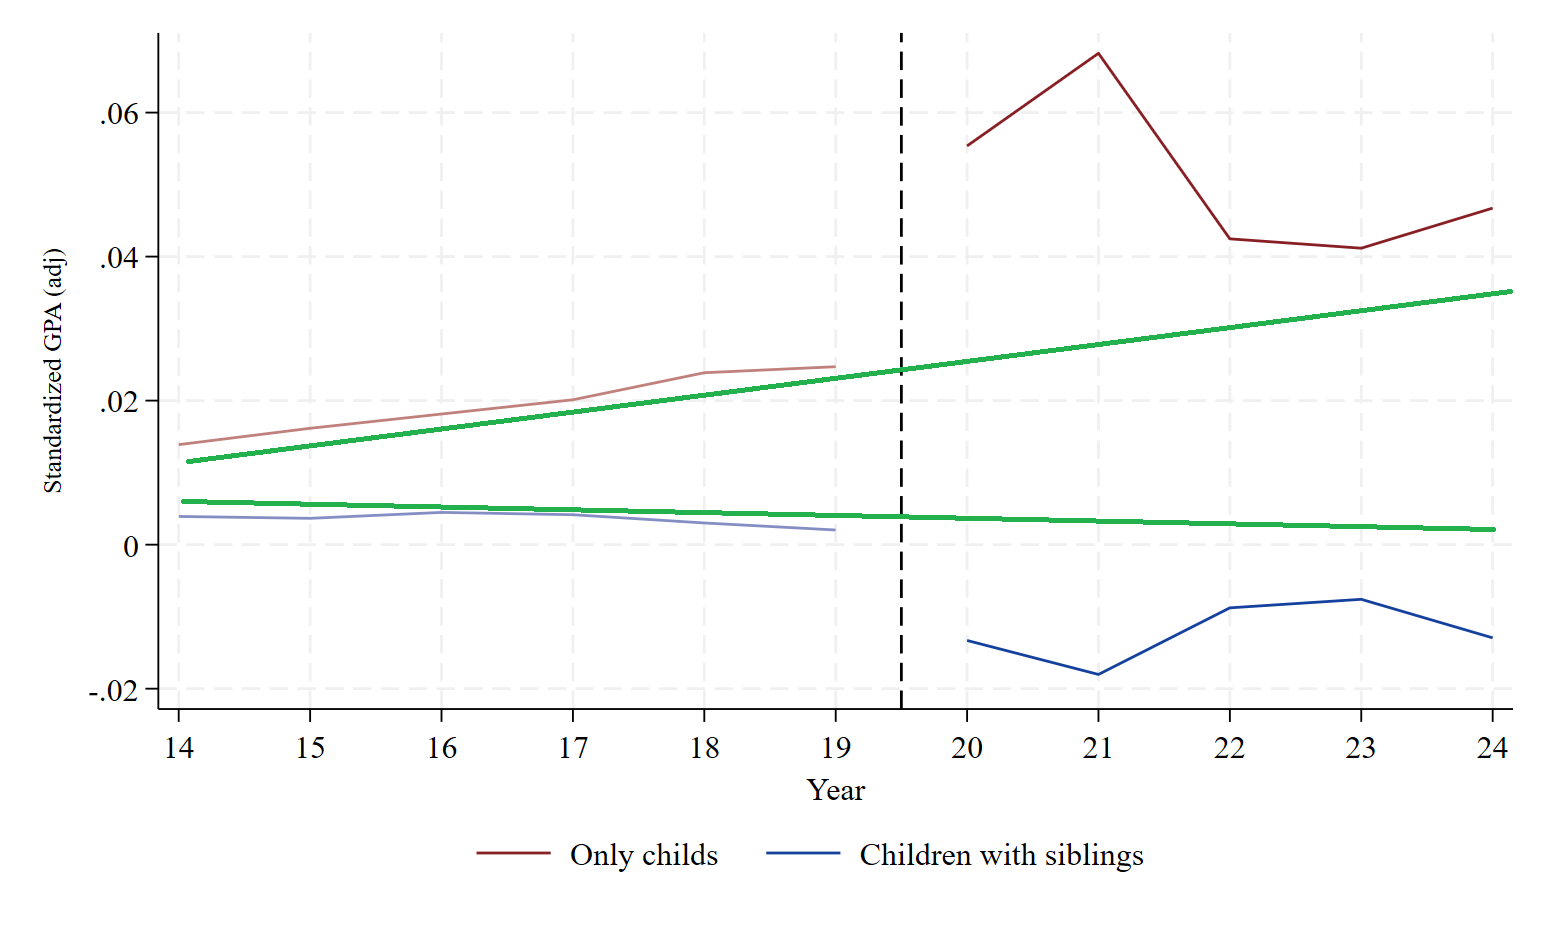
\includegraphics{./FIGURES/Descriptive/parallel_trends.png}
      }
    }
\end{frame}



\begin{frame}
    \label{update_scott}
    \frametitle{Raw plots per cohort - Age trend}
        {\resizebox{0.9\textwidth}{!}{
       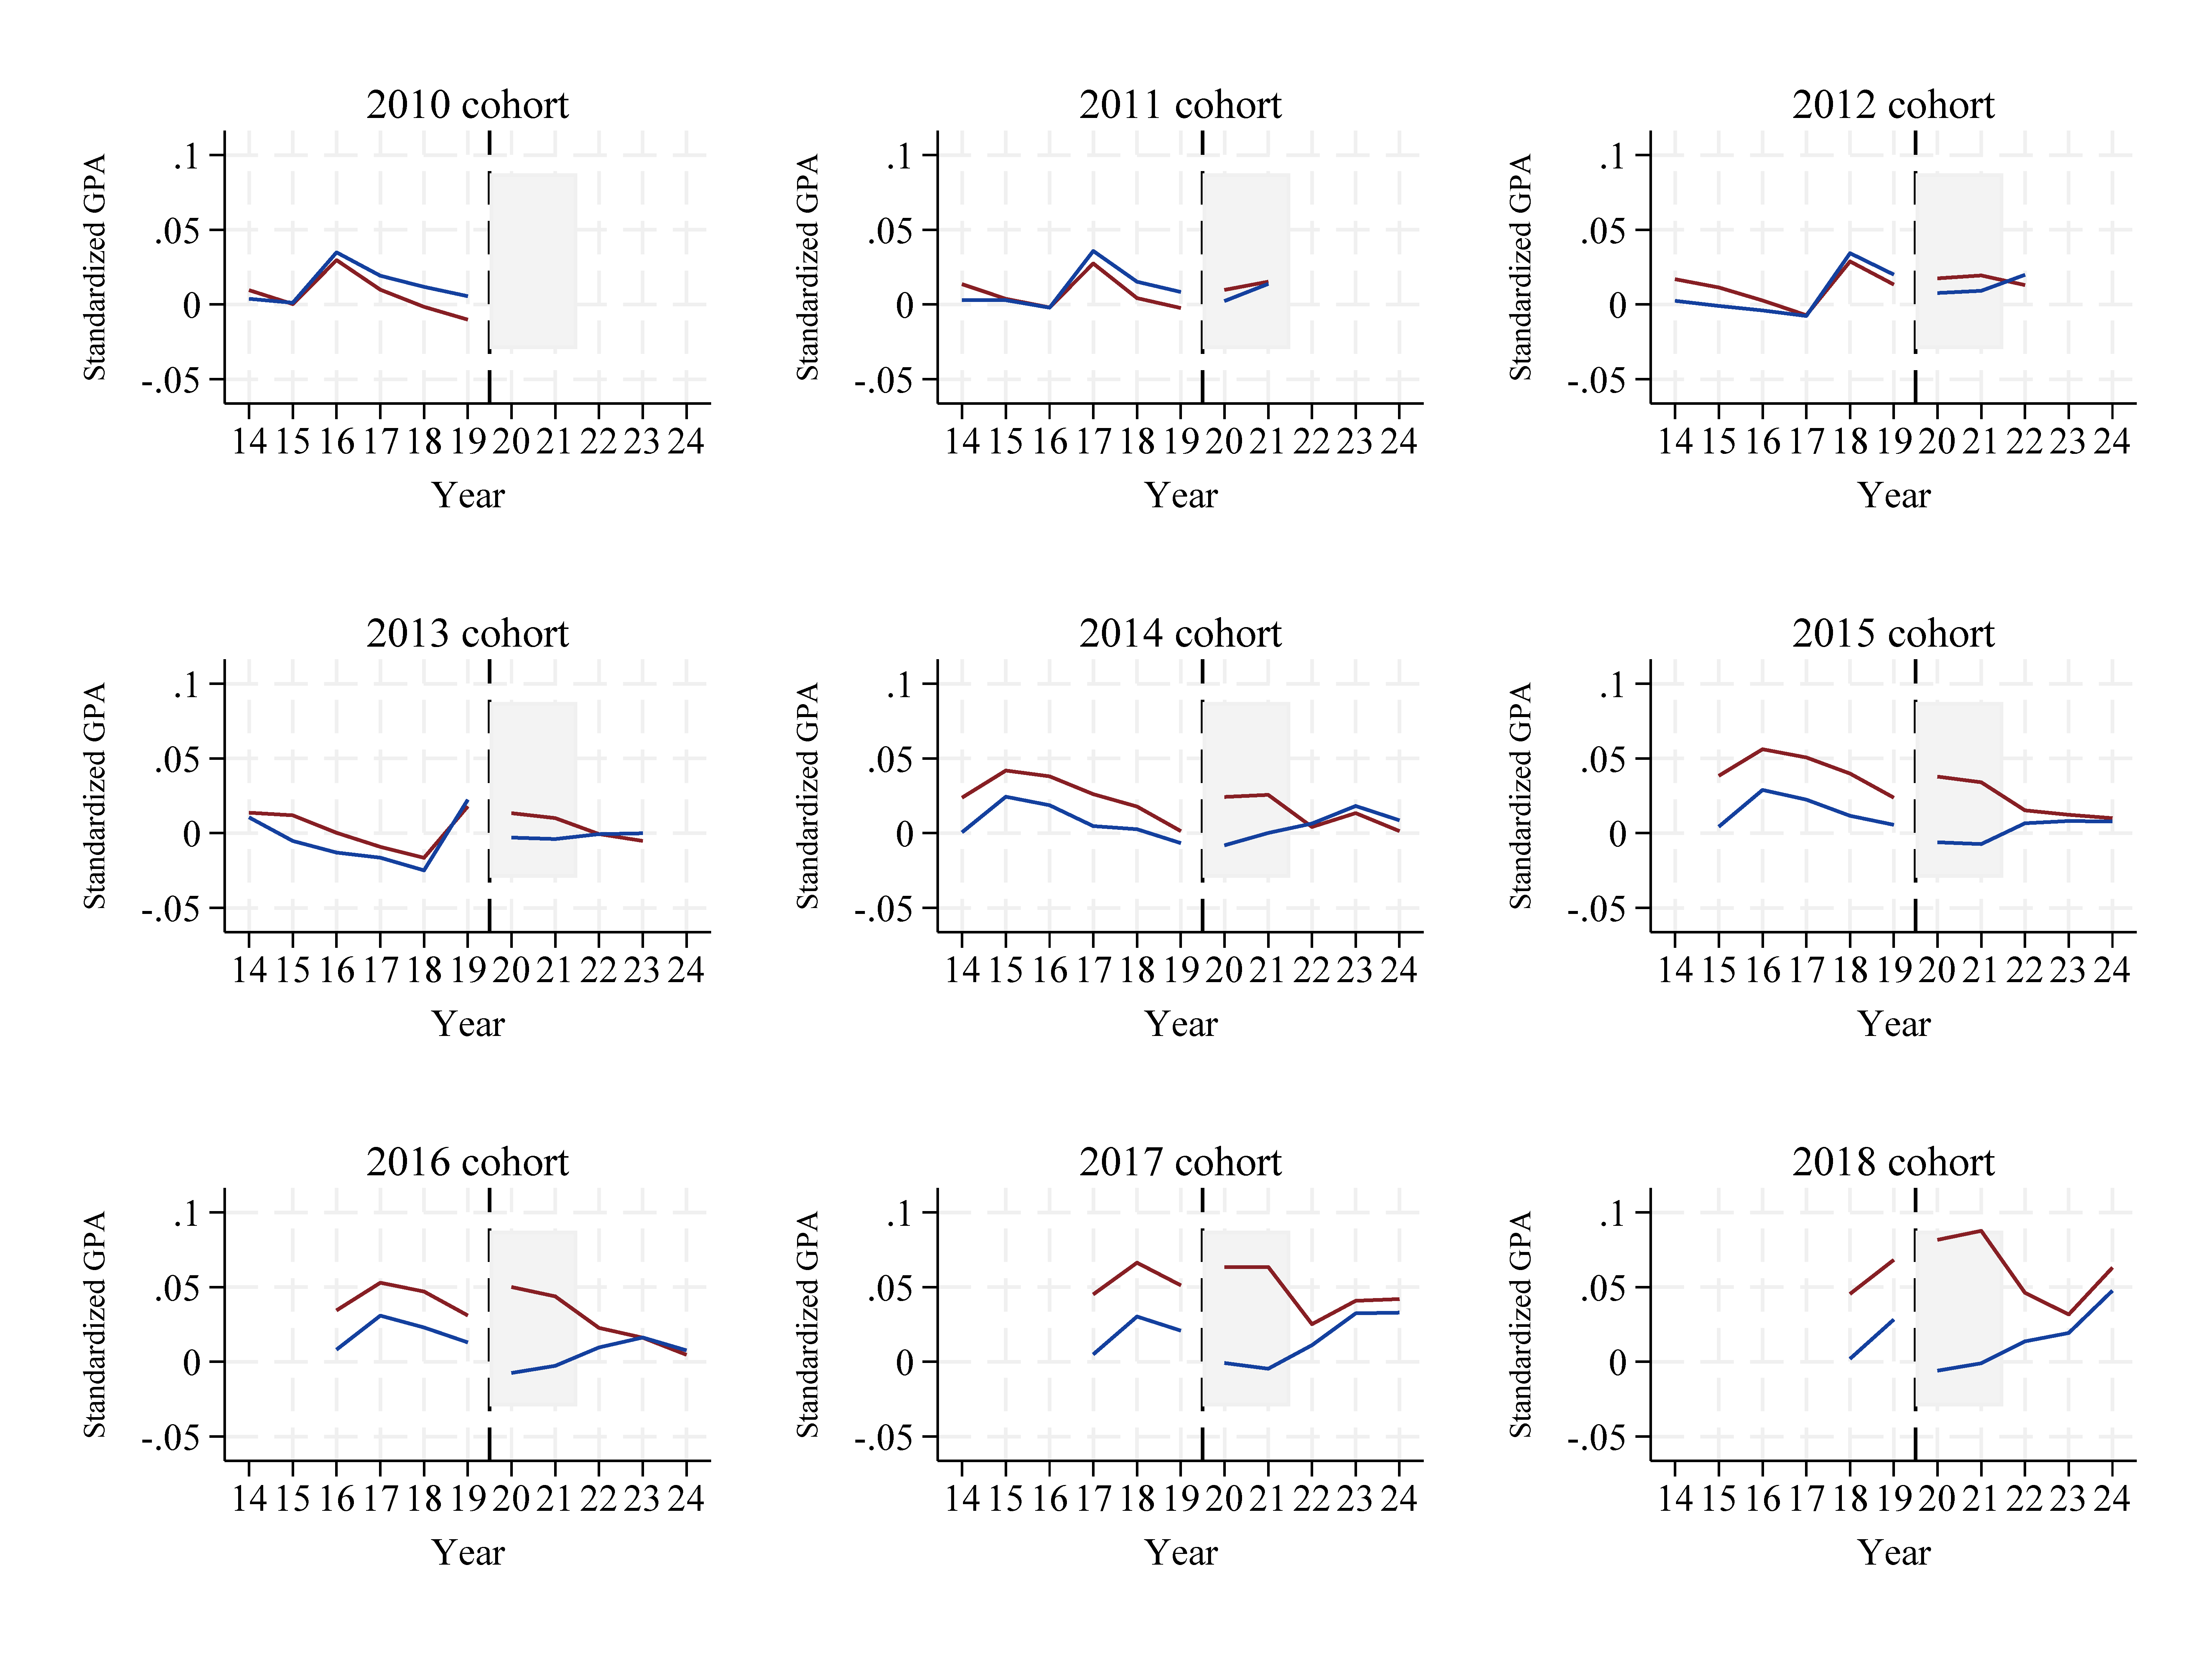
\includegraphics{./FIGURES/Descriptive/raw_cohorts_std_gpa_m.pdf}
      }
    }
\end{frame}

\begin{frame}
    \label{update_scott}
    \frametitle{Raw plots per grade - Time trend}
        {\resizebox{0.8\textwidth}{!}{
       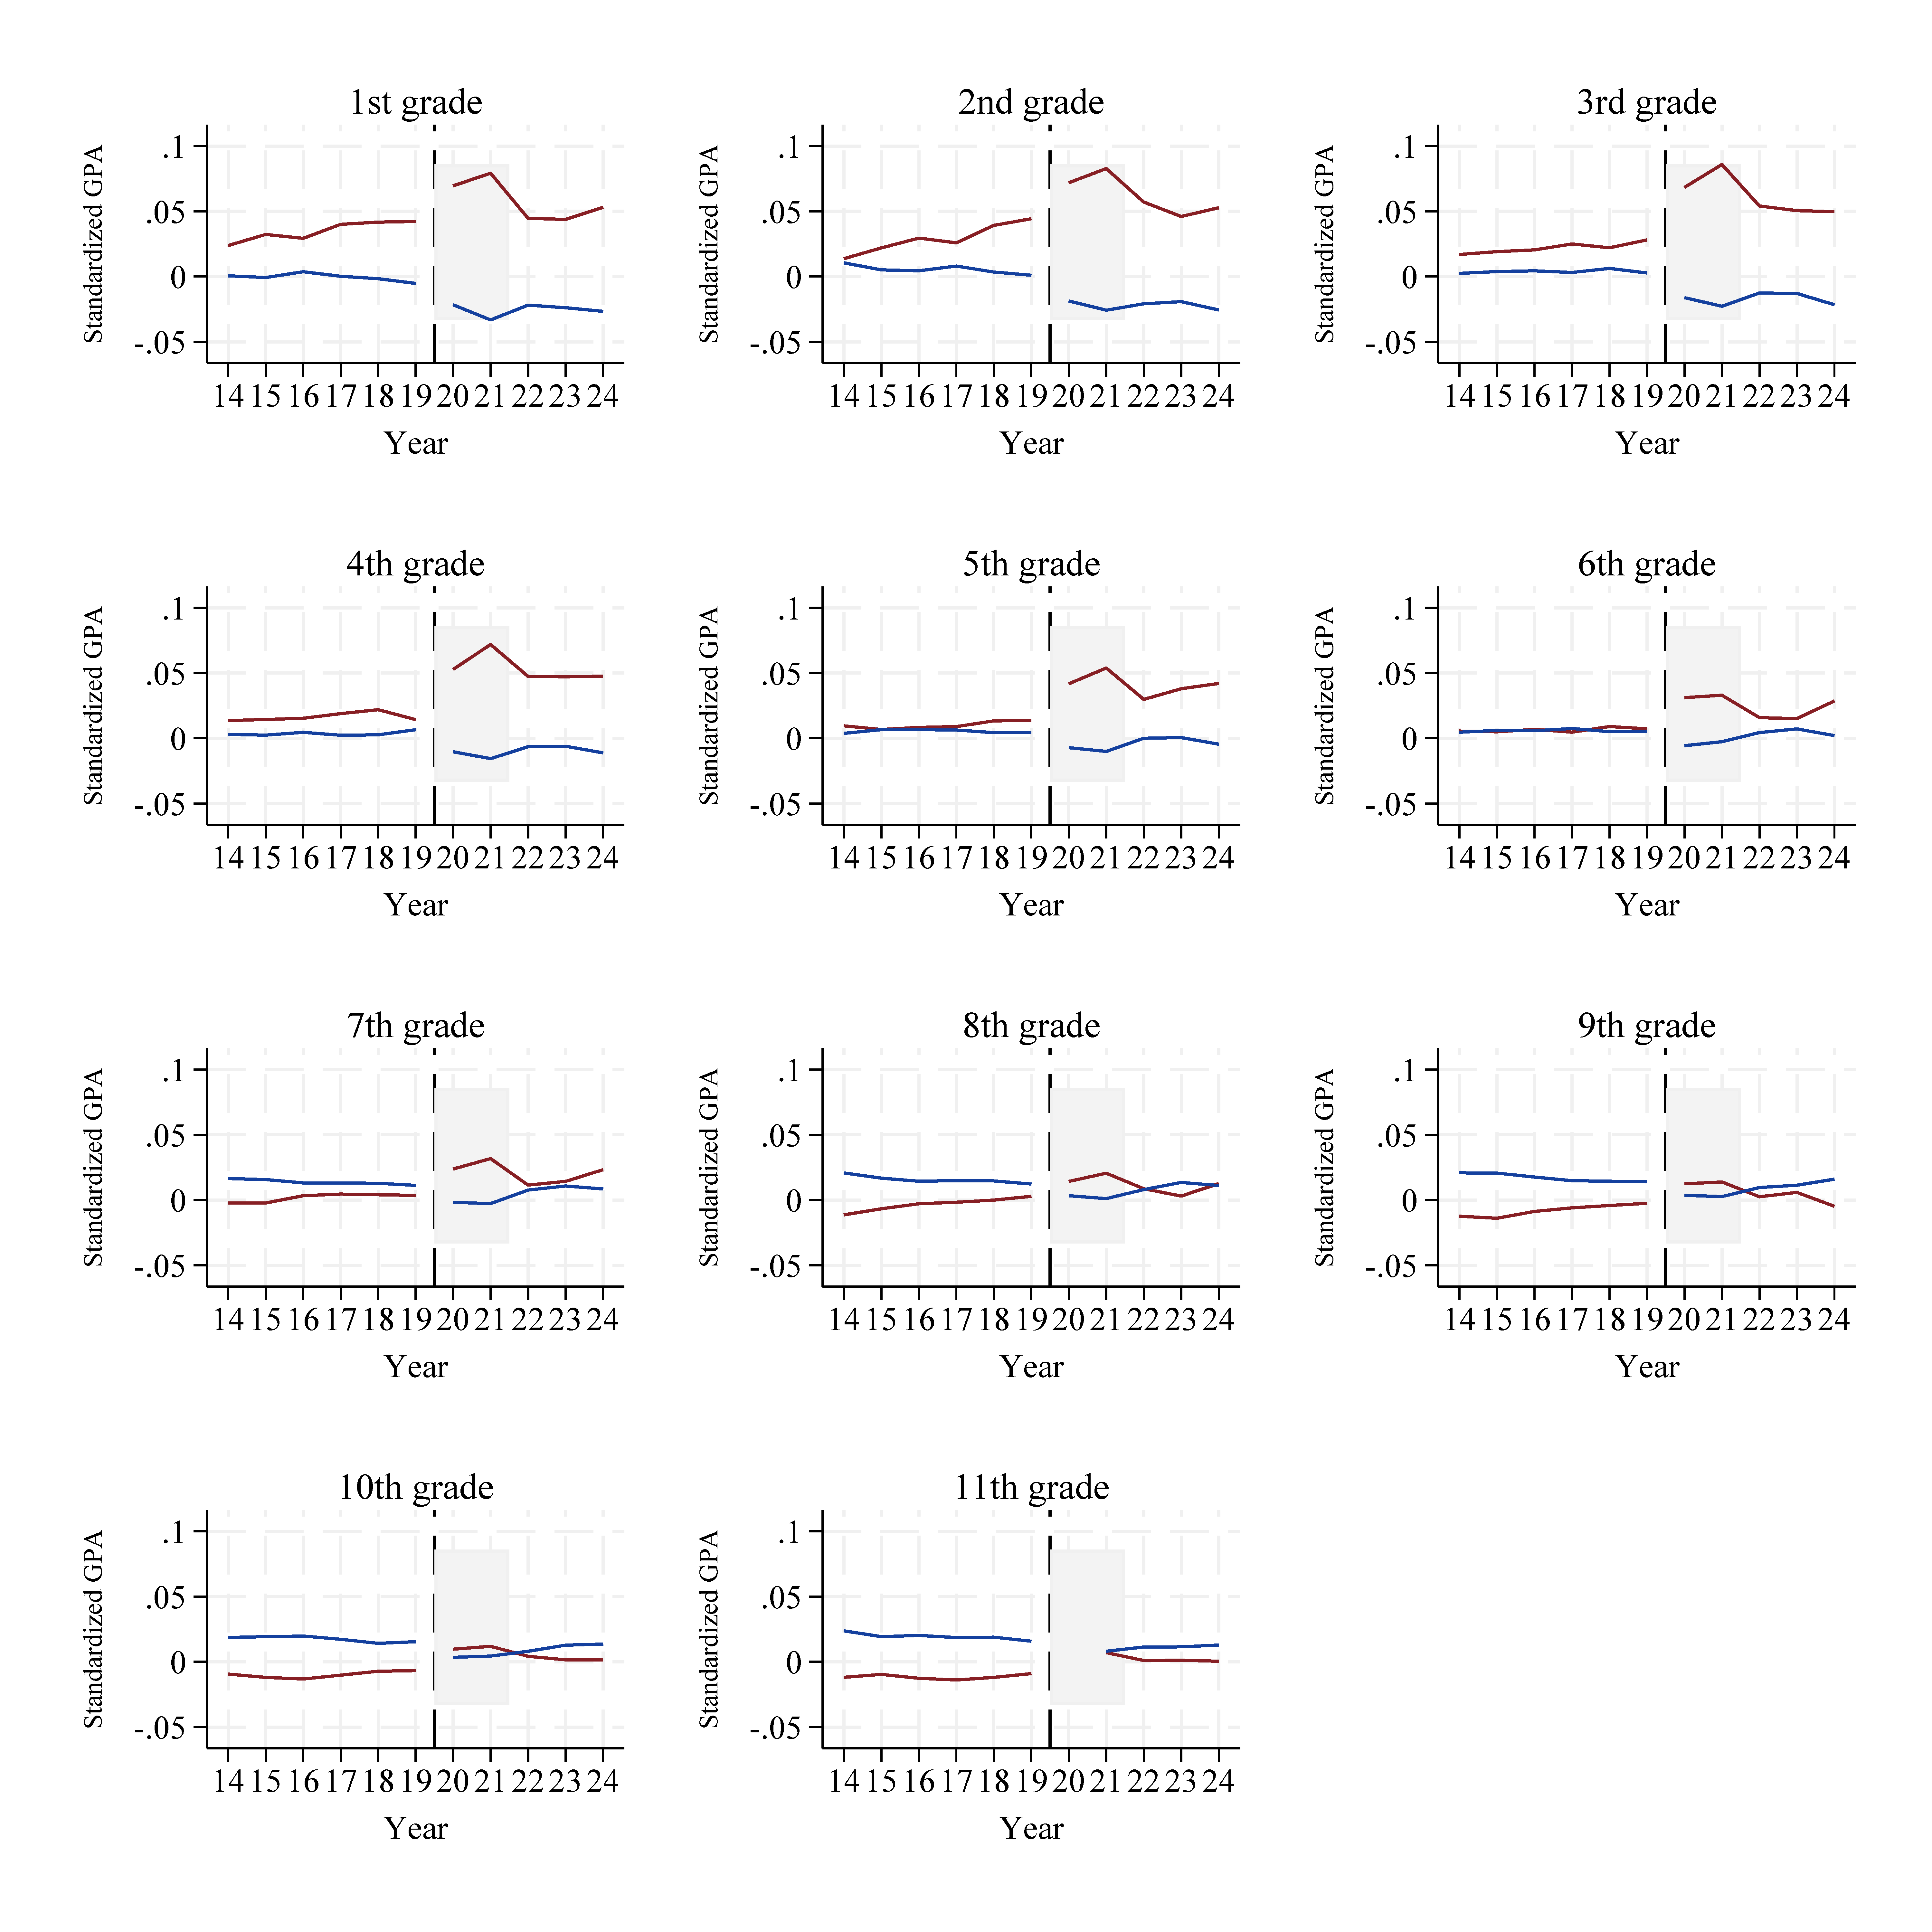
\includegraphics{./FIGURES/Descriptive/raw_grades_std_gpa_m.pdf}
      }
    }
\end{frame}

\begin{frame}
    \label{update_scott}
    \frametitle{TWFE}
 {\resizebox{0.9\textwidth}{!}{
       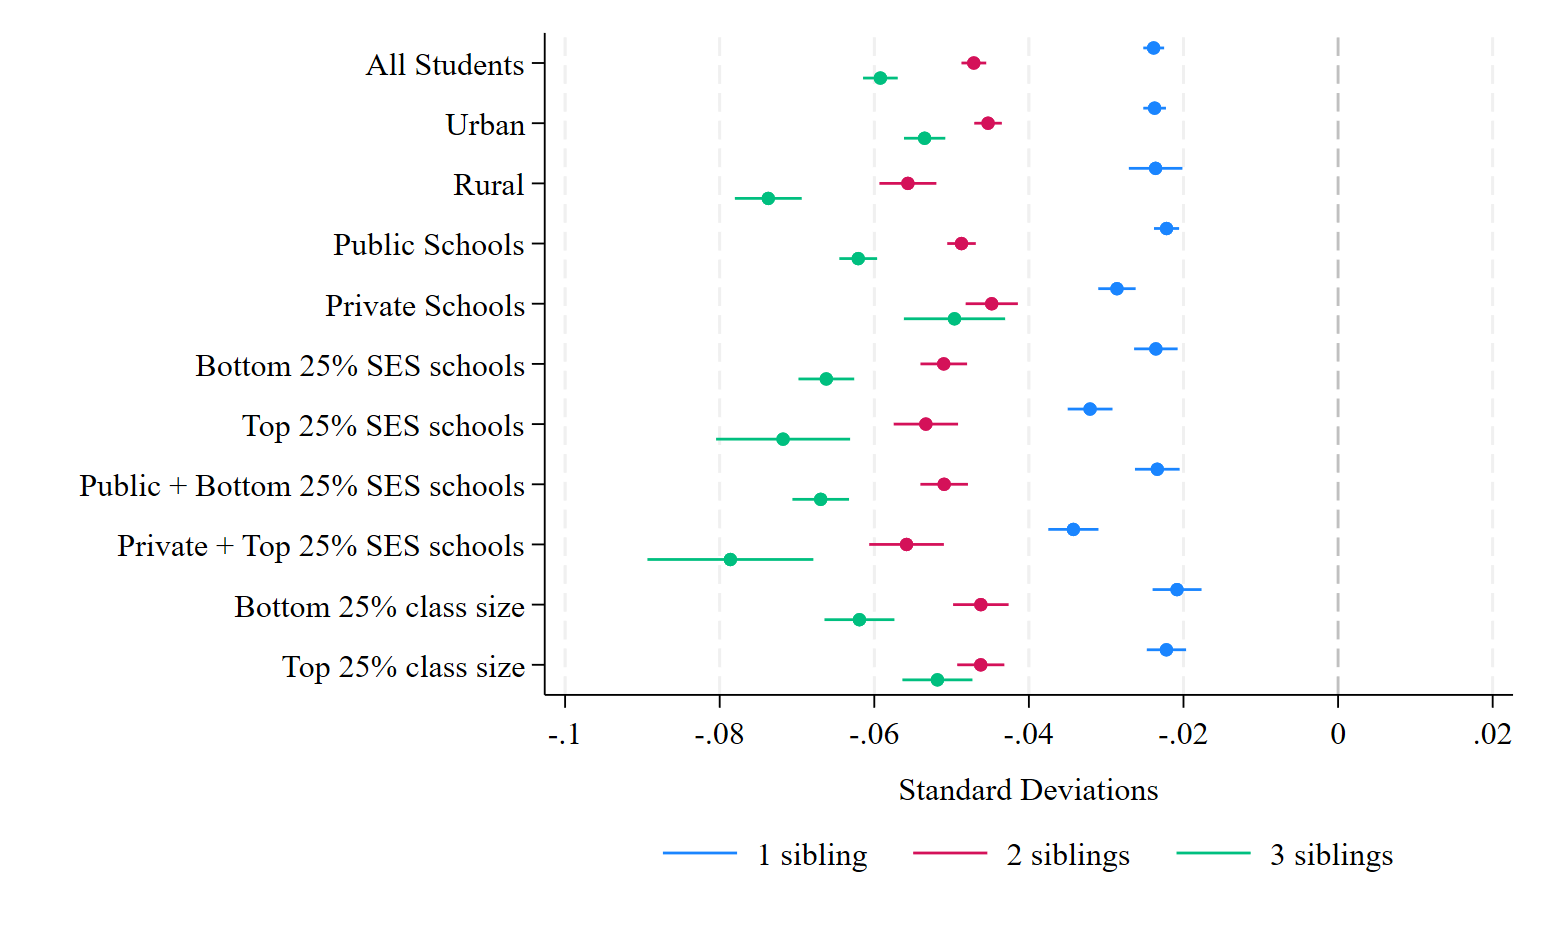
\includegraphics{./FIGURES/TWFE/covid_twfe_A_all_gpa_m_4.png}
      }
    }
\end{frame}

\begin{frame}
    \label{update_scott}
    \frametitle{TWFE}
 {\resizebox{0.9\textwidth}{!}{
       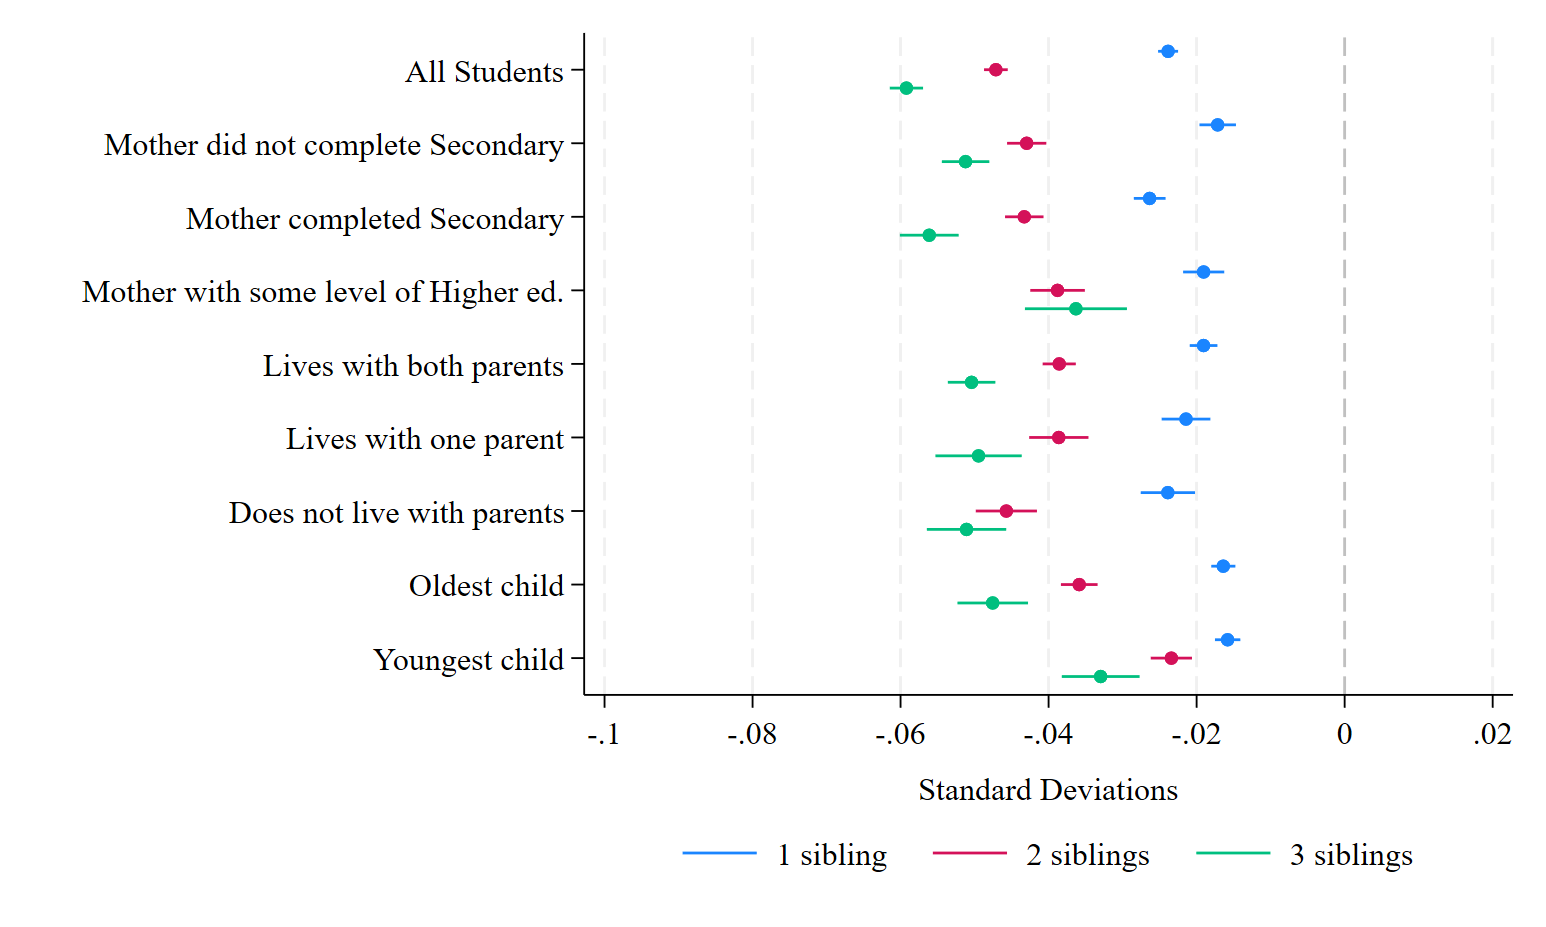
\includegraphics{./FIGURES/TWFE/covid_twfe_B_all_gpa_m_4.png}
      }
    }
\end{frame}


\begin{frame}
    \label{update_scott}
    \frametitle{School average standardized exams - 2nd grade}
        {\resizebox{0.9\textwidth}{!}{
       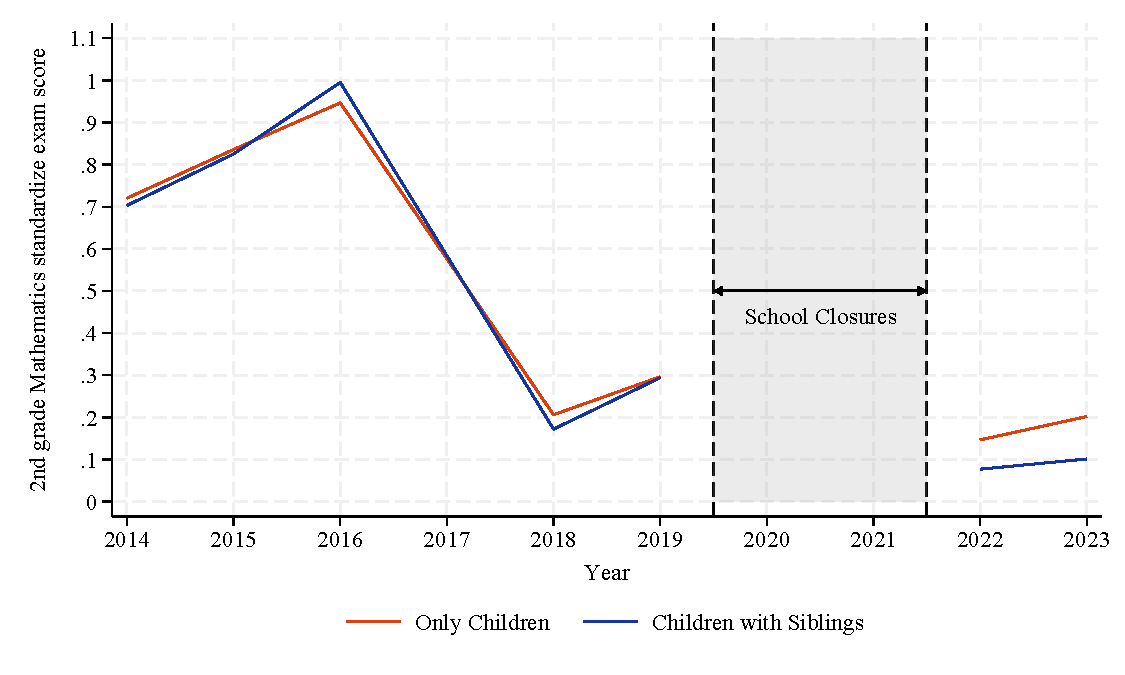
\includegraphics{./FIGURES/Descriptive/raw_ece_math_2.pdf}
      }
    }
\end{frame}

\begin{frame}
    \label{update_scott}
    \frametitle{School average standardized exams - 4th grade}
        {\resizebox{0.9\textwidth}{!}{
       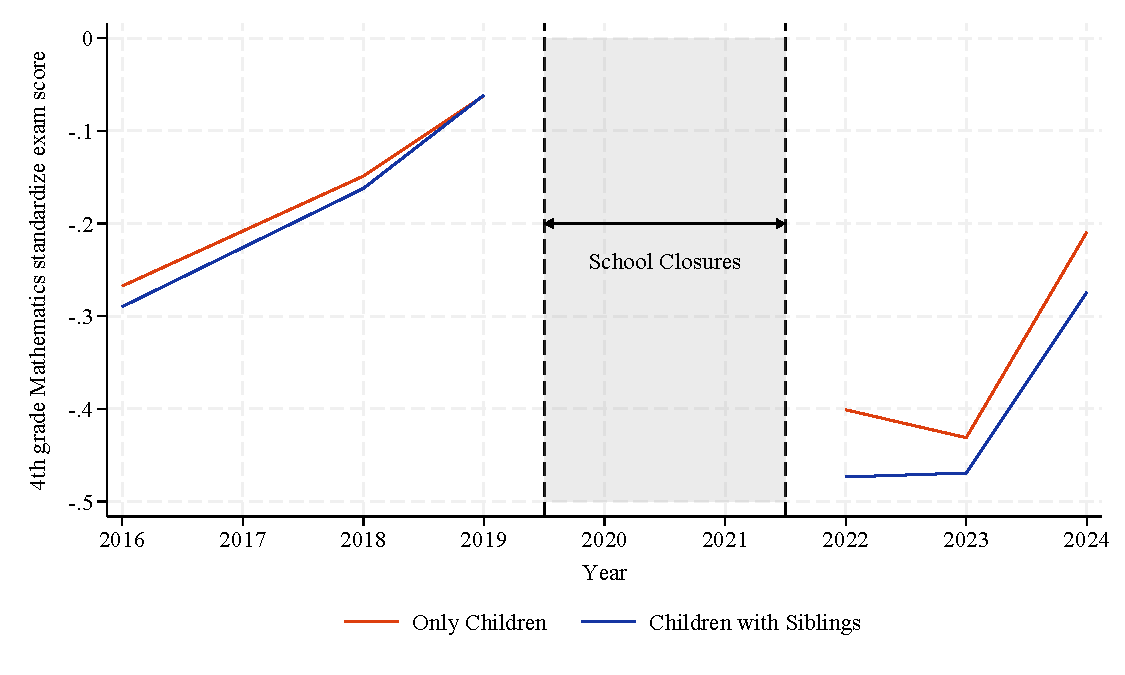
\includegraphics{./FIGURES/Descriptive/raw_ece_math_4.pdf}
      }
    }
\end{frame}

\begin{frame}
    \label{update_scott}
    \frametitle{School average standardized exams - 8th grade}
        {\resizebox{0.9\textwidth}{!}{
       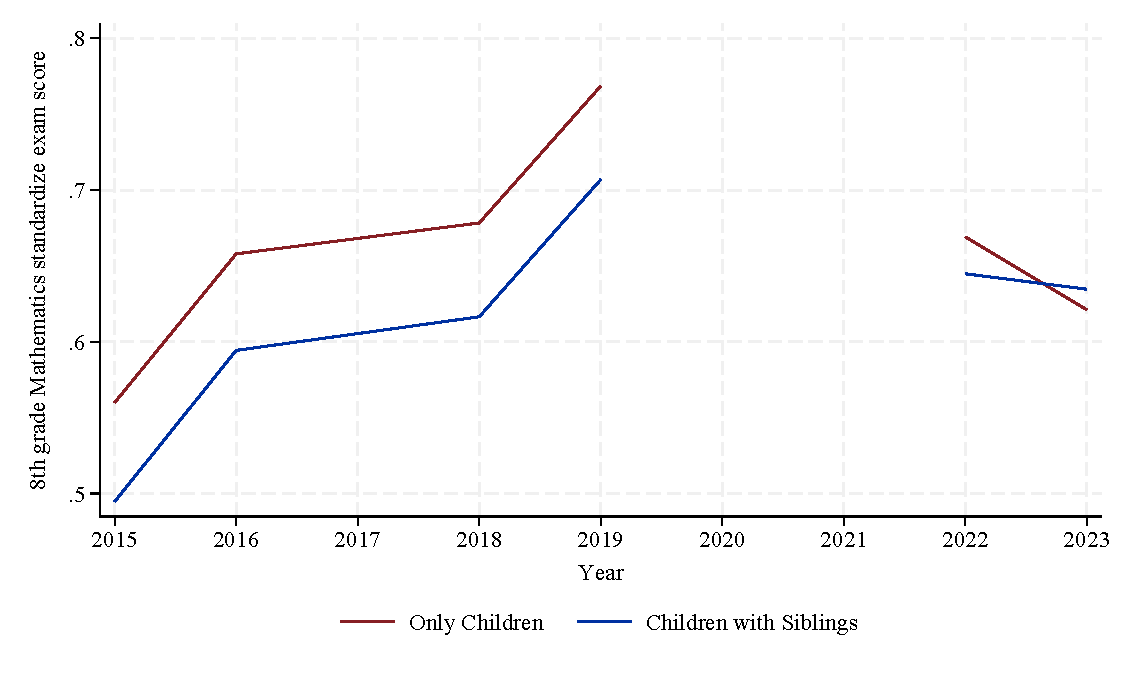
\includegraphics{./FIGURES/Descriptive/raw_ece_math_8.pdf}
      }
    }
\end{frame}


\begin{frame}
    \label{update_scott}
    \frametitle{Event Study - 2nd grade}
 {\resizebox{0.9\textwidth}{!}{
       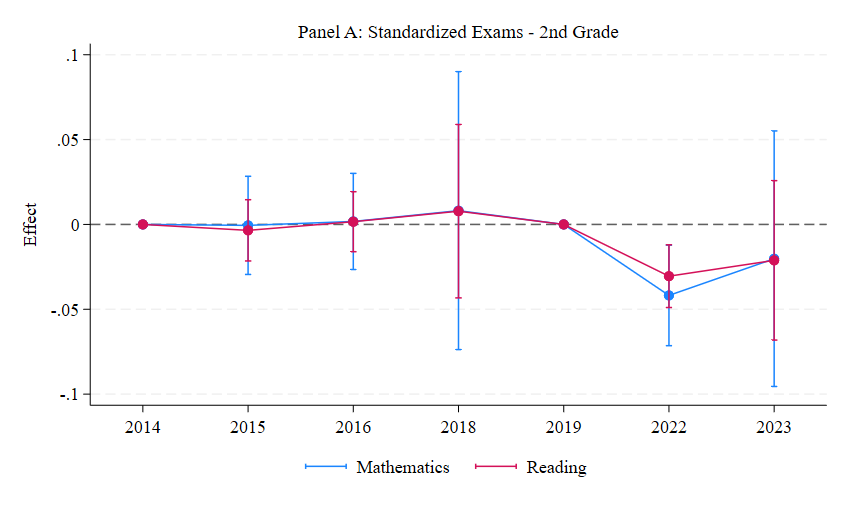
\includegraphics{./FIGURES/Event Study/ece_school_score_2p.png}
      }
    }
\end{frame}


\begin{frame}
    \label{update_scott}
    \frametitle{Event Study - 4th grade}
 {\resizebox{0.9\textwidth}{!}{
       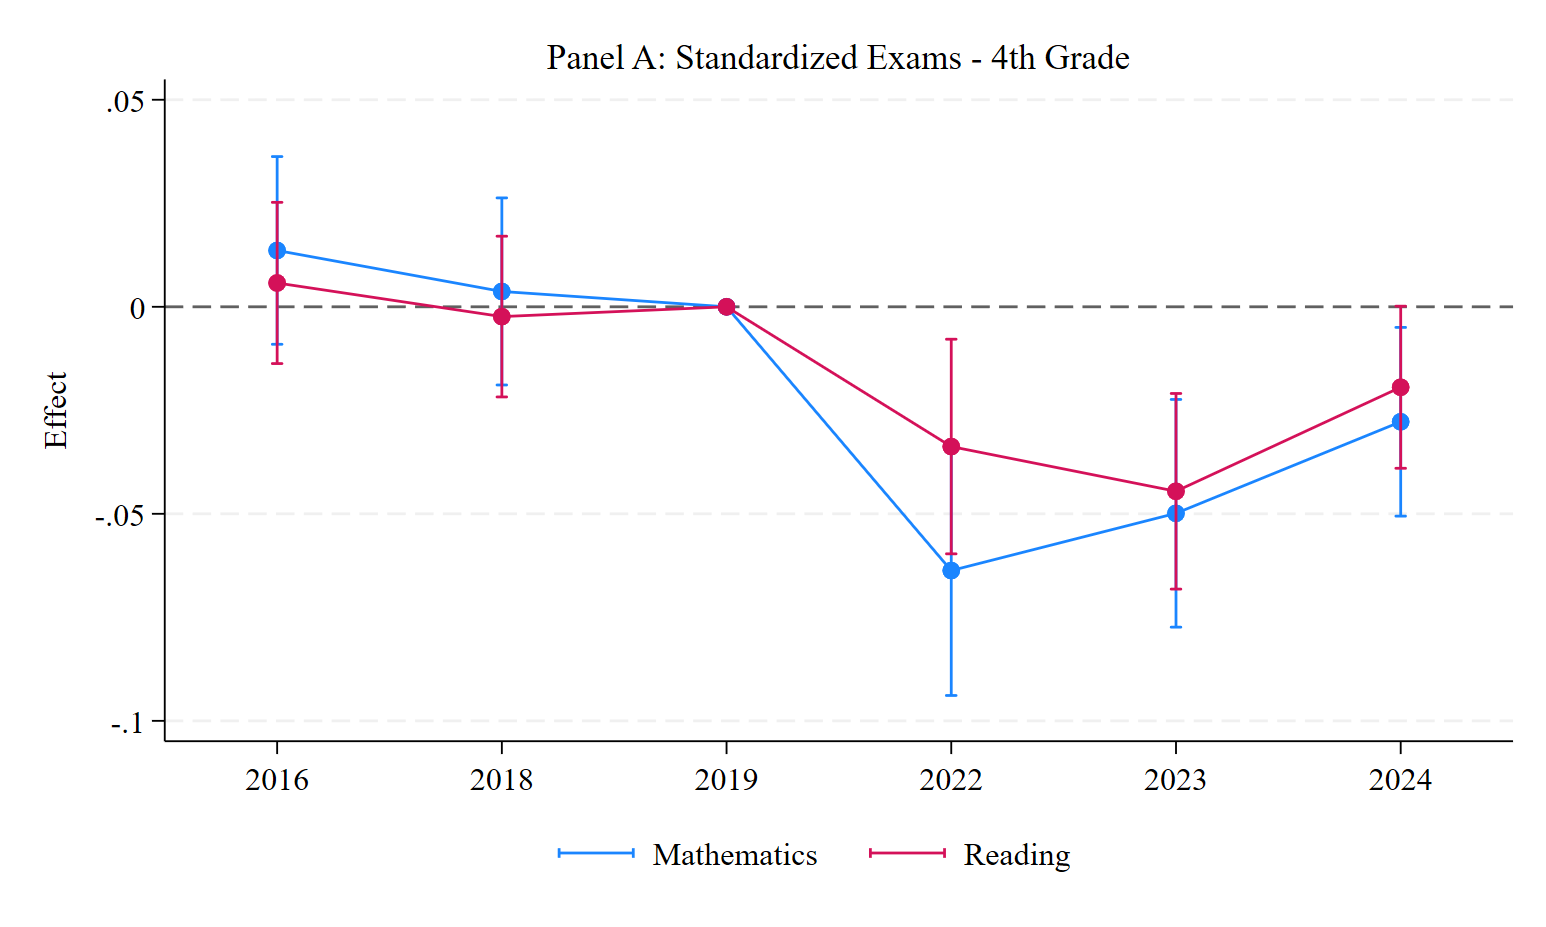
\includegraphics{./FIGURES/Event Study/ece_school_score_4p.png}
      }
    }
\end{frame}


\begin{frame}
    \label{update_scott}
    \frametitle{Event Study - 8th grade}
 {\resizebox{0.9\textwidth}{!}{
       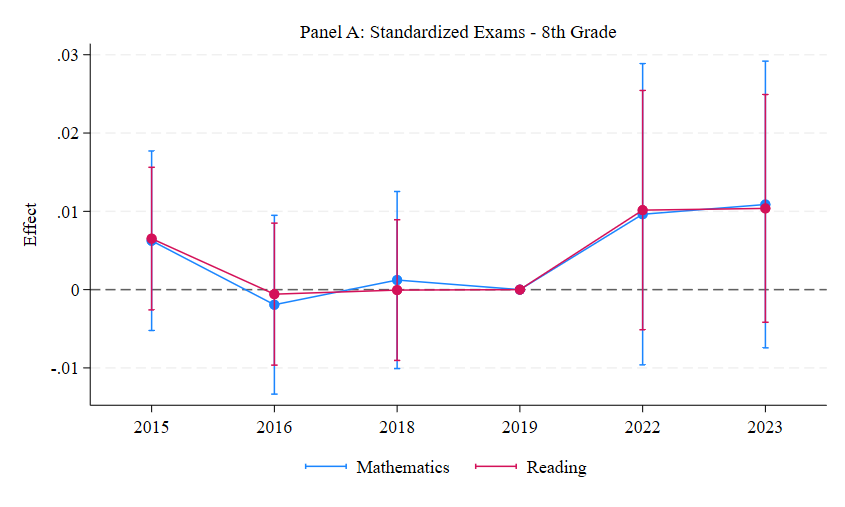
\includegraphics{./FIGURES/Event Study/ece_school_score_2s.png}
      }
    }
\end{frame}


\begin{frame}
    \label{event_cohort_m}
    \frametitle{Evidence from the Netherlands}
    \begin{itemize}
        \item Had 2 school closures during 1.5 years of Covid. $\approx$ 8 weeks of closure.
        \item Studies heterogeneity by SES, single parents, # of siblings (1-2, vs 3+). Find effects on the first, not on # of siblings.
        \item Look at learning growth across different cohorts
   
       $\Delta Y_{ijc}= \beta Post + \epsilon_{ijc}$ 
       $\Delta Y_{ijc}= \beta Post + \gamma SES + \delta Post*SES + \epsilon_{ijc}$ 
     \end{itemize}
\end{frame}


\begin{frame}
    \label{update_scott}
    \frametitle{Grade thresholds during covid}
    \begin{itemize}
        \item During covid (full academic year 2020 and 2021) all children were promoted and no subject was failed. 
        \item D grade was elimiated and grades went from 0-20 to 11-20.
        \item This could cause an spurious effect if one population was more likely below the passing grade
    \end{itemize}
\end{frame}


\begin{frame}
    \label{update_scott}
    \frametitle{Grade distributions pre-covid: Elementary}
 {\resizebox{0.9\textwidth}{!}{
       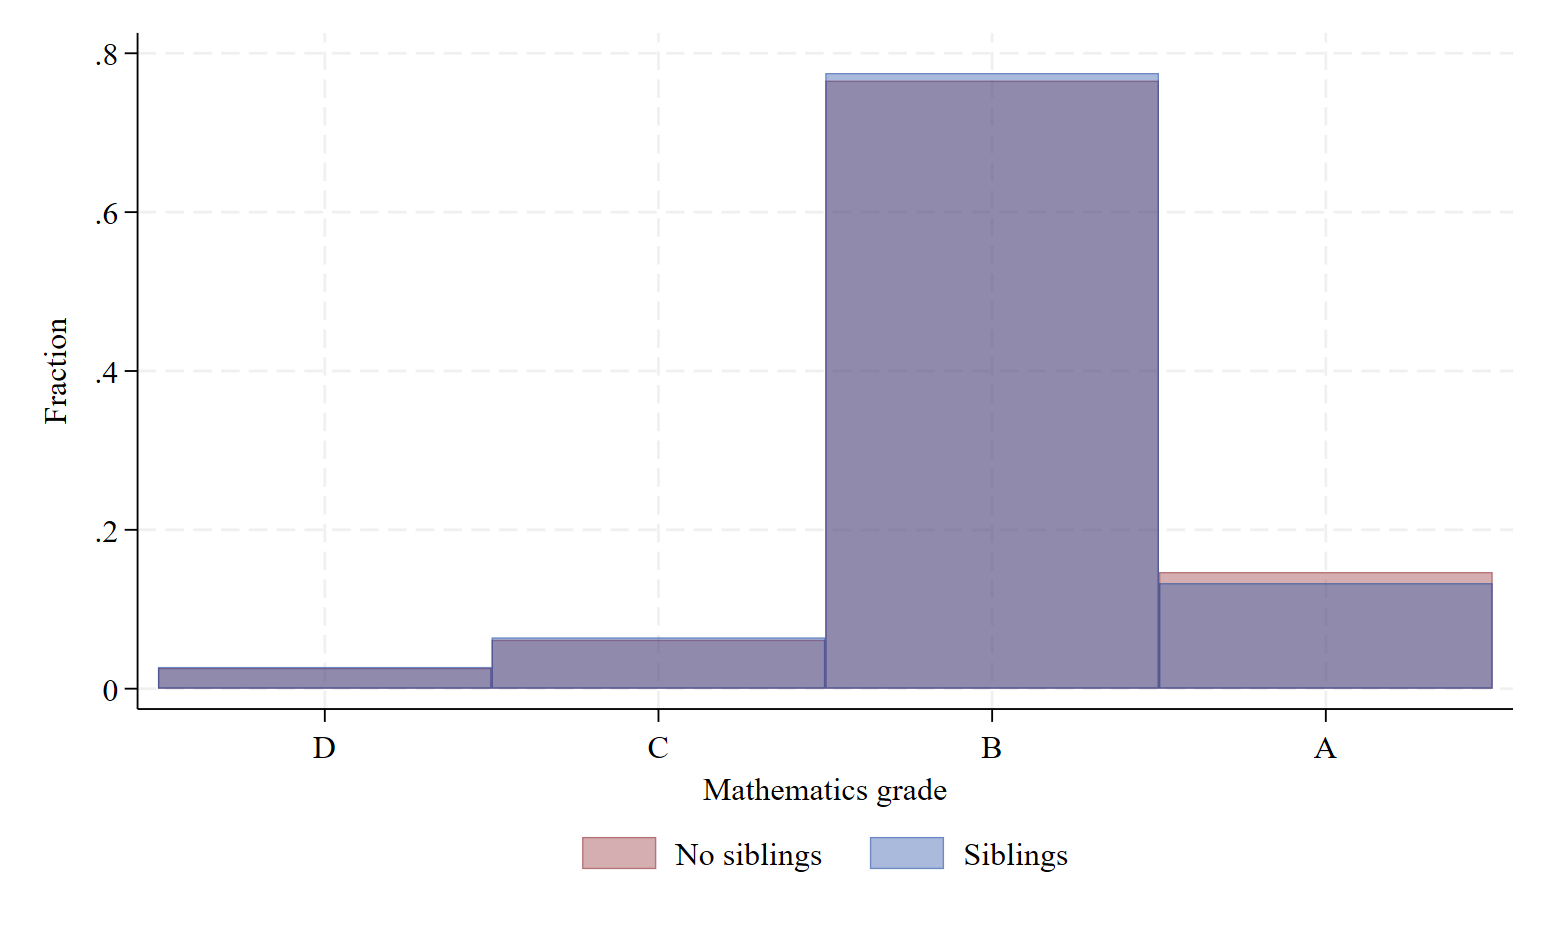
\includegraphics{./FIGURES/Descriptive/histogram_pre_elm.png}
      }
    }
\end{frame}

\begin{frame}
    \label{update_scott}
    \frametitle{Grade distributions pre-covid: Secondary}
 {\resizebox{0.9\textwidth}{!}{
       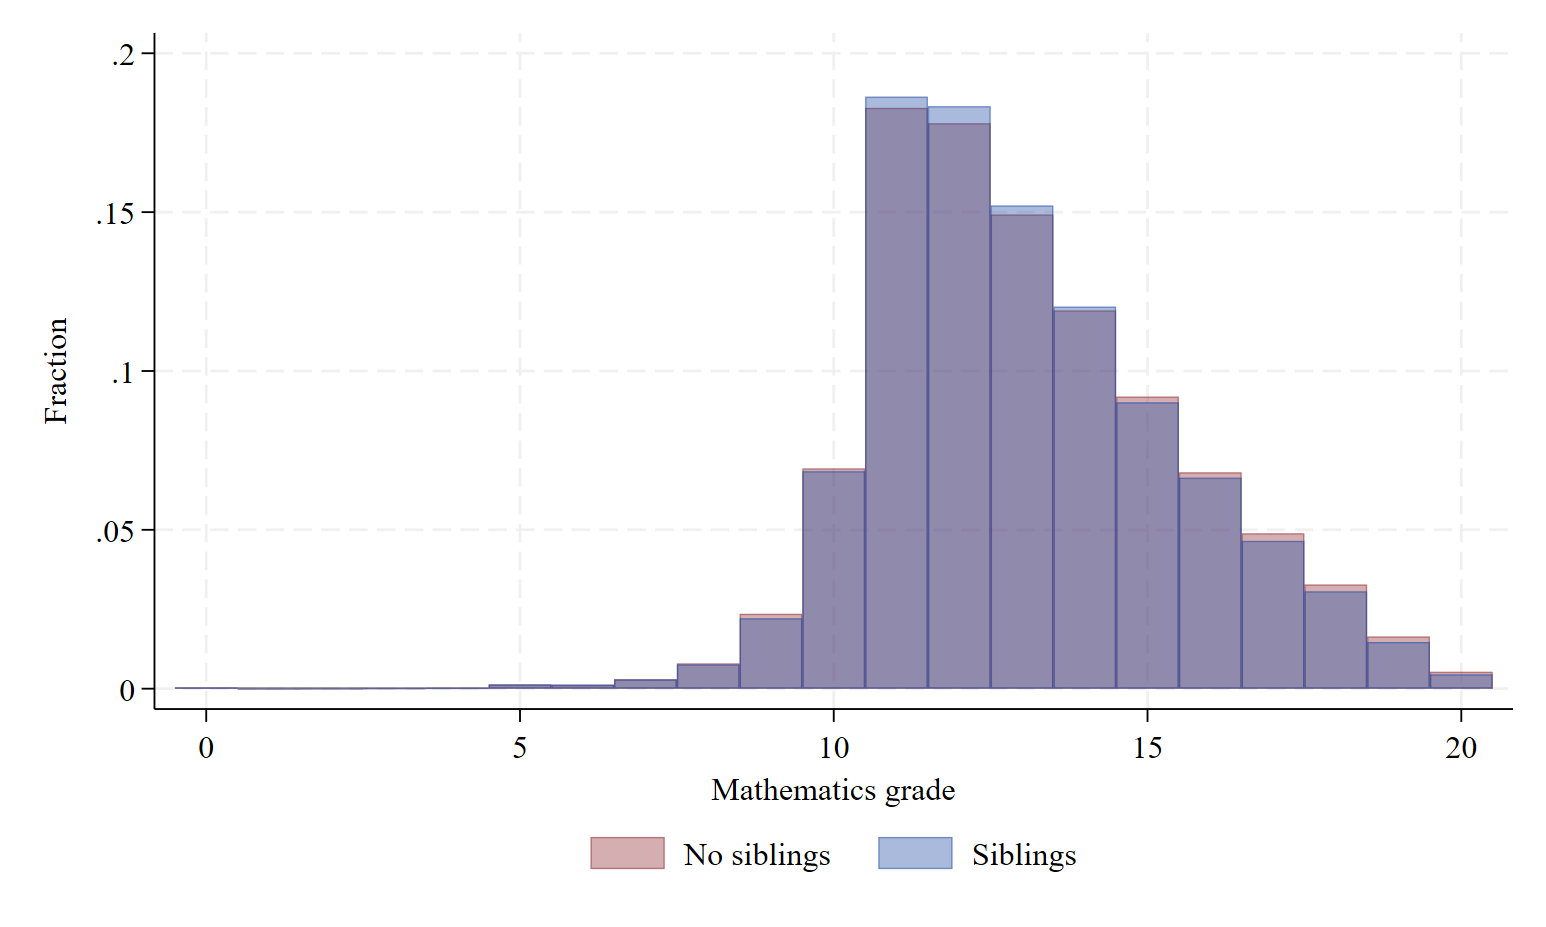
\includegraphics{./FIGURES/Descriptive/histogram_pre_9-10.png}
      }
    }
\end{frame}

\begin{frame}
    \label{update_scott}
    \frametitle{Grade distributions post-covid: Elementary}
 {\resizebox{0.9\textwidth}{!}{
       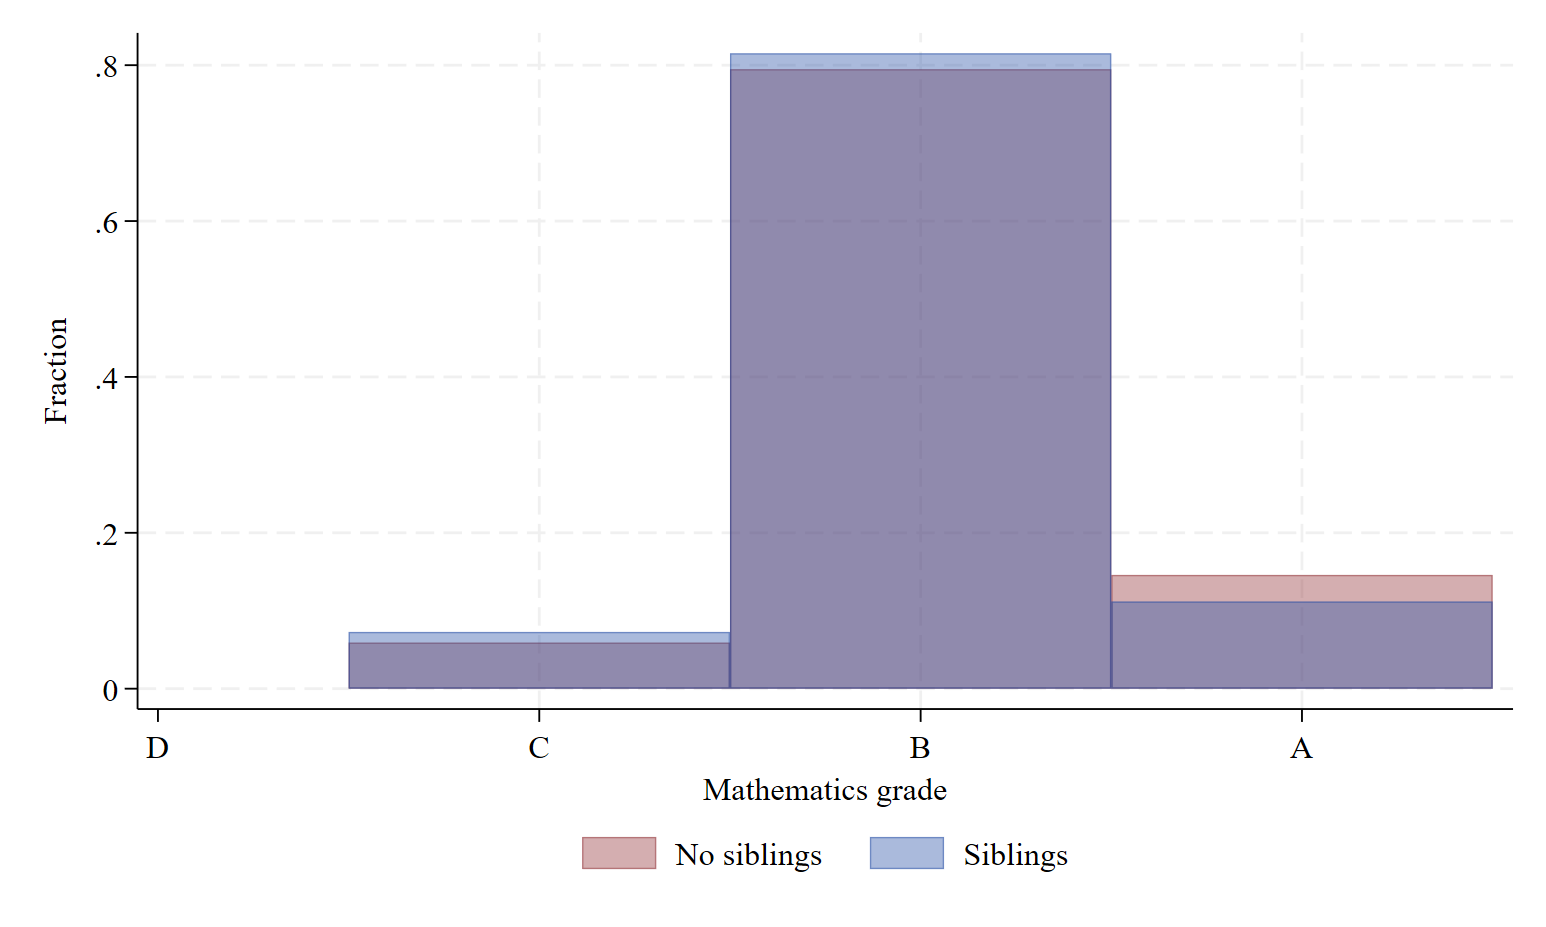
\includegraphics{./FIGURES/Descriptive/histogram_post_elm.png}
      }
    }
\end{frame}

\begin{frame}
    \label{update_scott}
    \frametitle{Grade distributions post-covid: Secondary}
 {\resizebox{0.9\textwidth}{!}{
       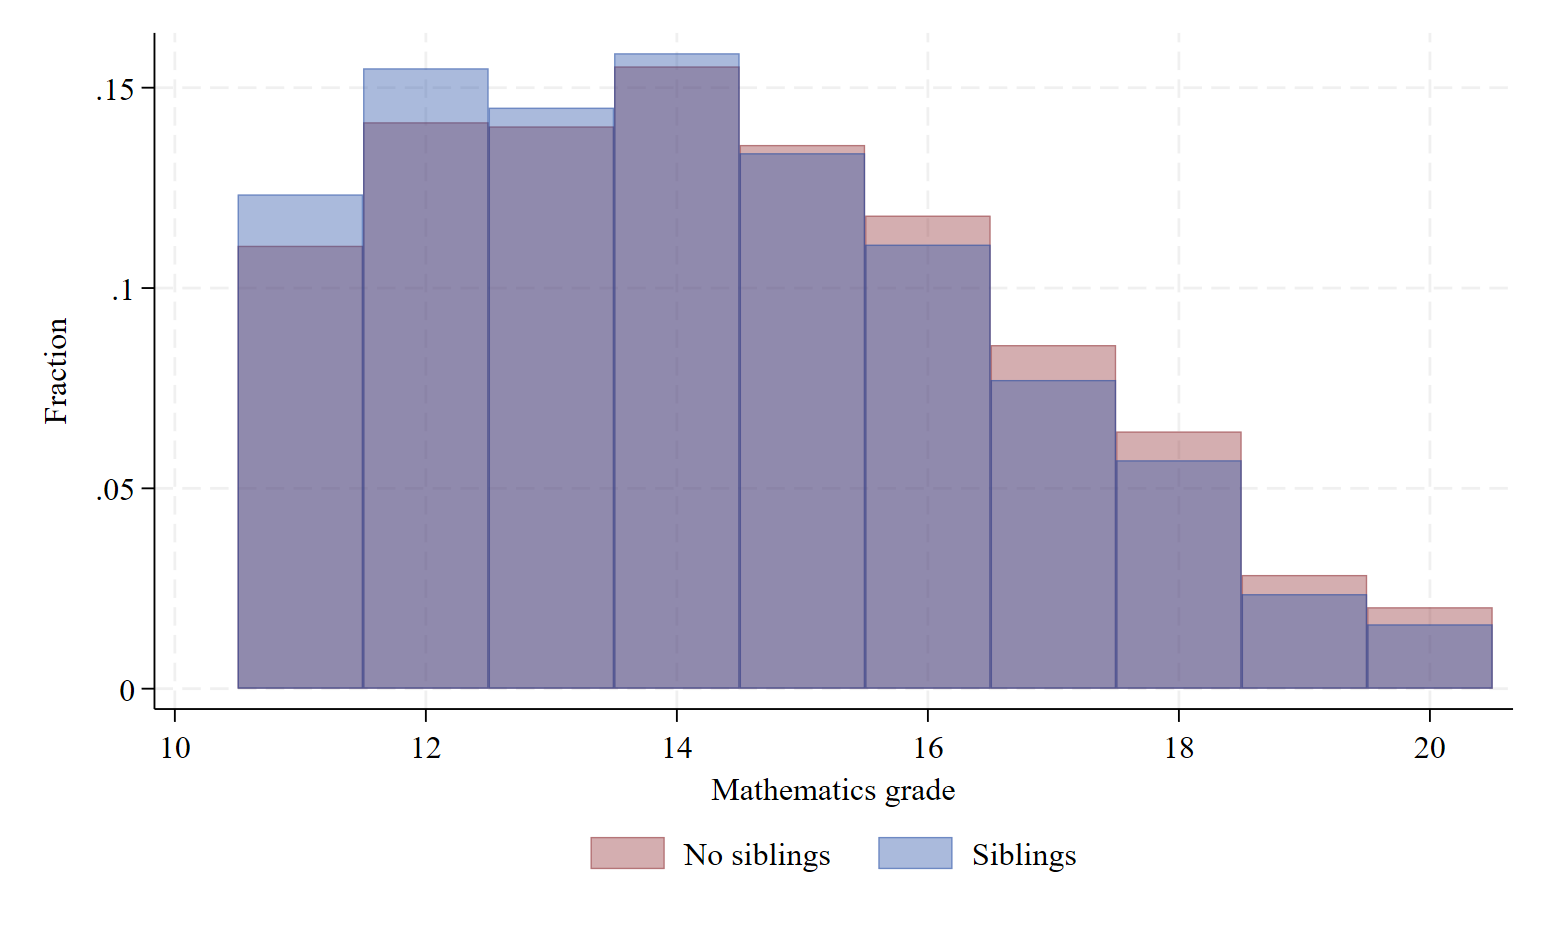
\includegraphics{./FIGURES/Descriptive/histogram_post_9-10.png}
      }
    }
\end{frame}


\end{document}